\section[Limits on $T\bar{T}$ production]{Limits on \boldmath{$T\bar{T}$} production}
Given that no significant excess is observed in the signal regions, upper limits at $95\%$ CL on the $T\bar{T}$  production cross section are set in several benchmark scenarios as a function of $m_{T}$ and are compared to the theoretical prediction.
The resulting lower limits on $m_{T}$ correspond to the central value of the theoretical cross section. The scenarios considered involve different assumptions on the decay branching ratios. The search in the 1-lepton channel is particularly sensitive to the benchmark scenario of ${\rm BR}(T\to Ht )=1$, while the 0-lepton channel instead is particularly sensitive to ${\rm BR}(T\to Zt )=1$, as shown in figure \ref{sec:vlq:fig:centlimit}. Both the 1-lepton and the 0-lepton searches have comparable sensitivity to the weak-isospin doublet and singlet scenarios. Therefore, their combination represents an improvement of $50-70$ $\gev$ on the expected $T$-quark mass exclusion over the individual searches. The corresponding limits obtained for the combination are shown in figure \ref{sec:vlq:fig:singdoub}.


\begin{figure}[h!]
\begin{subfigure}{0.5\textwidth}
  \centering
  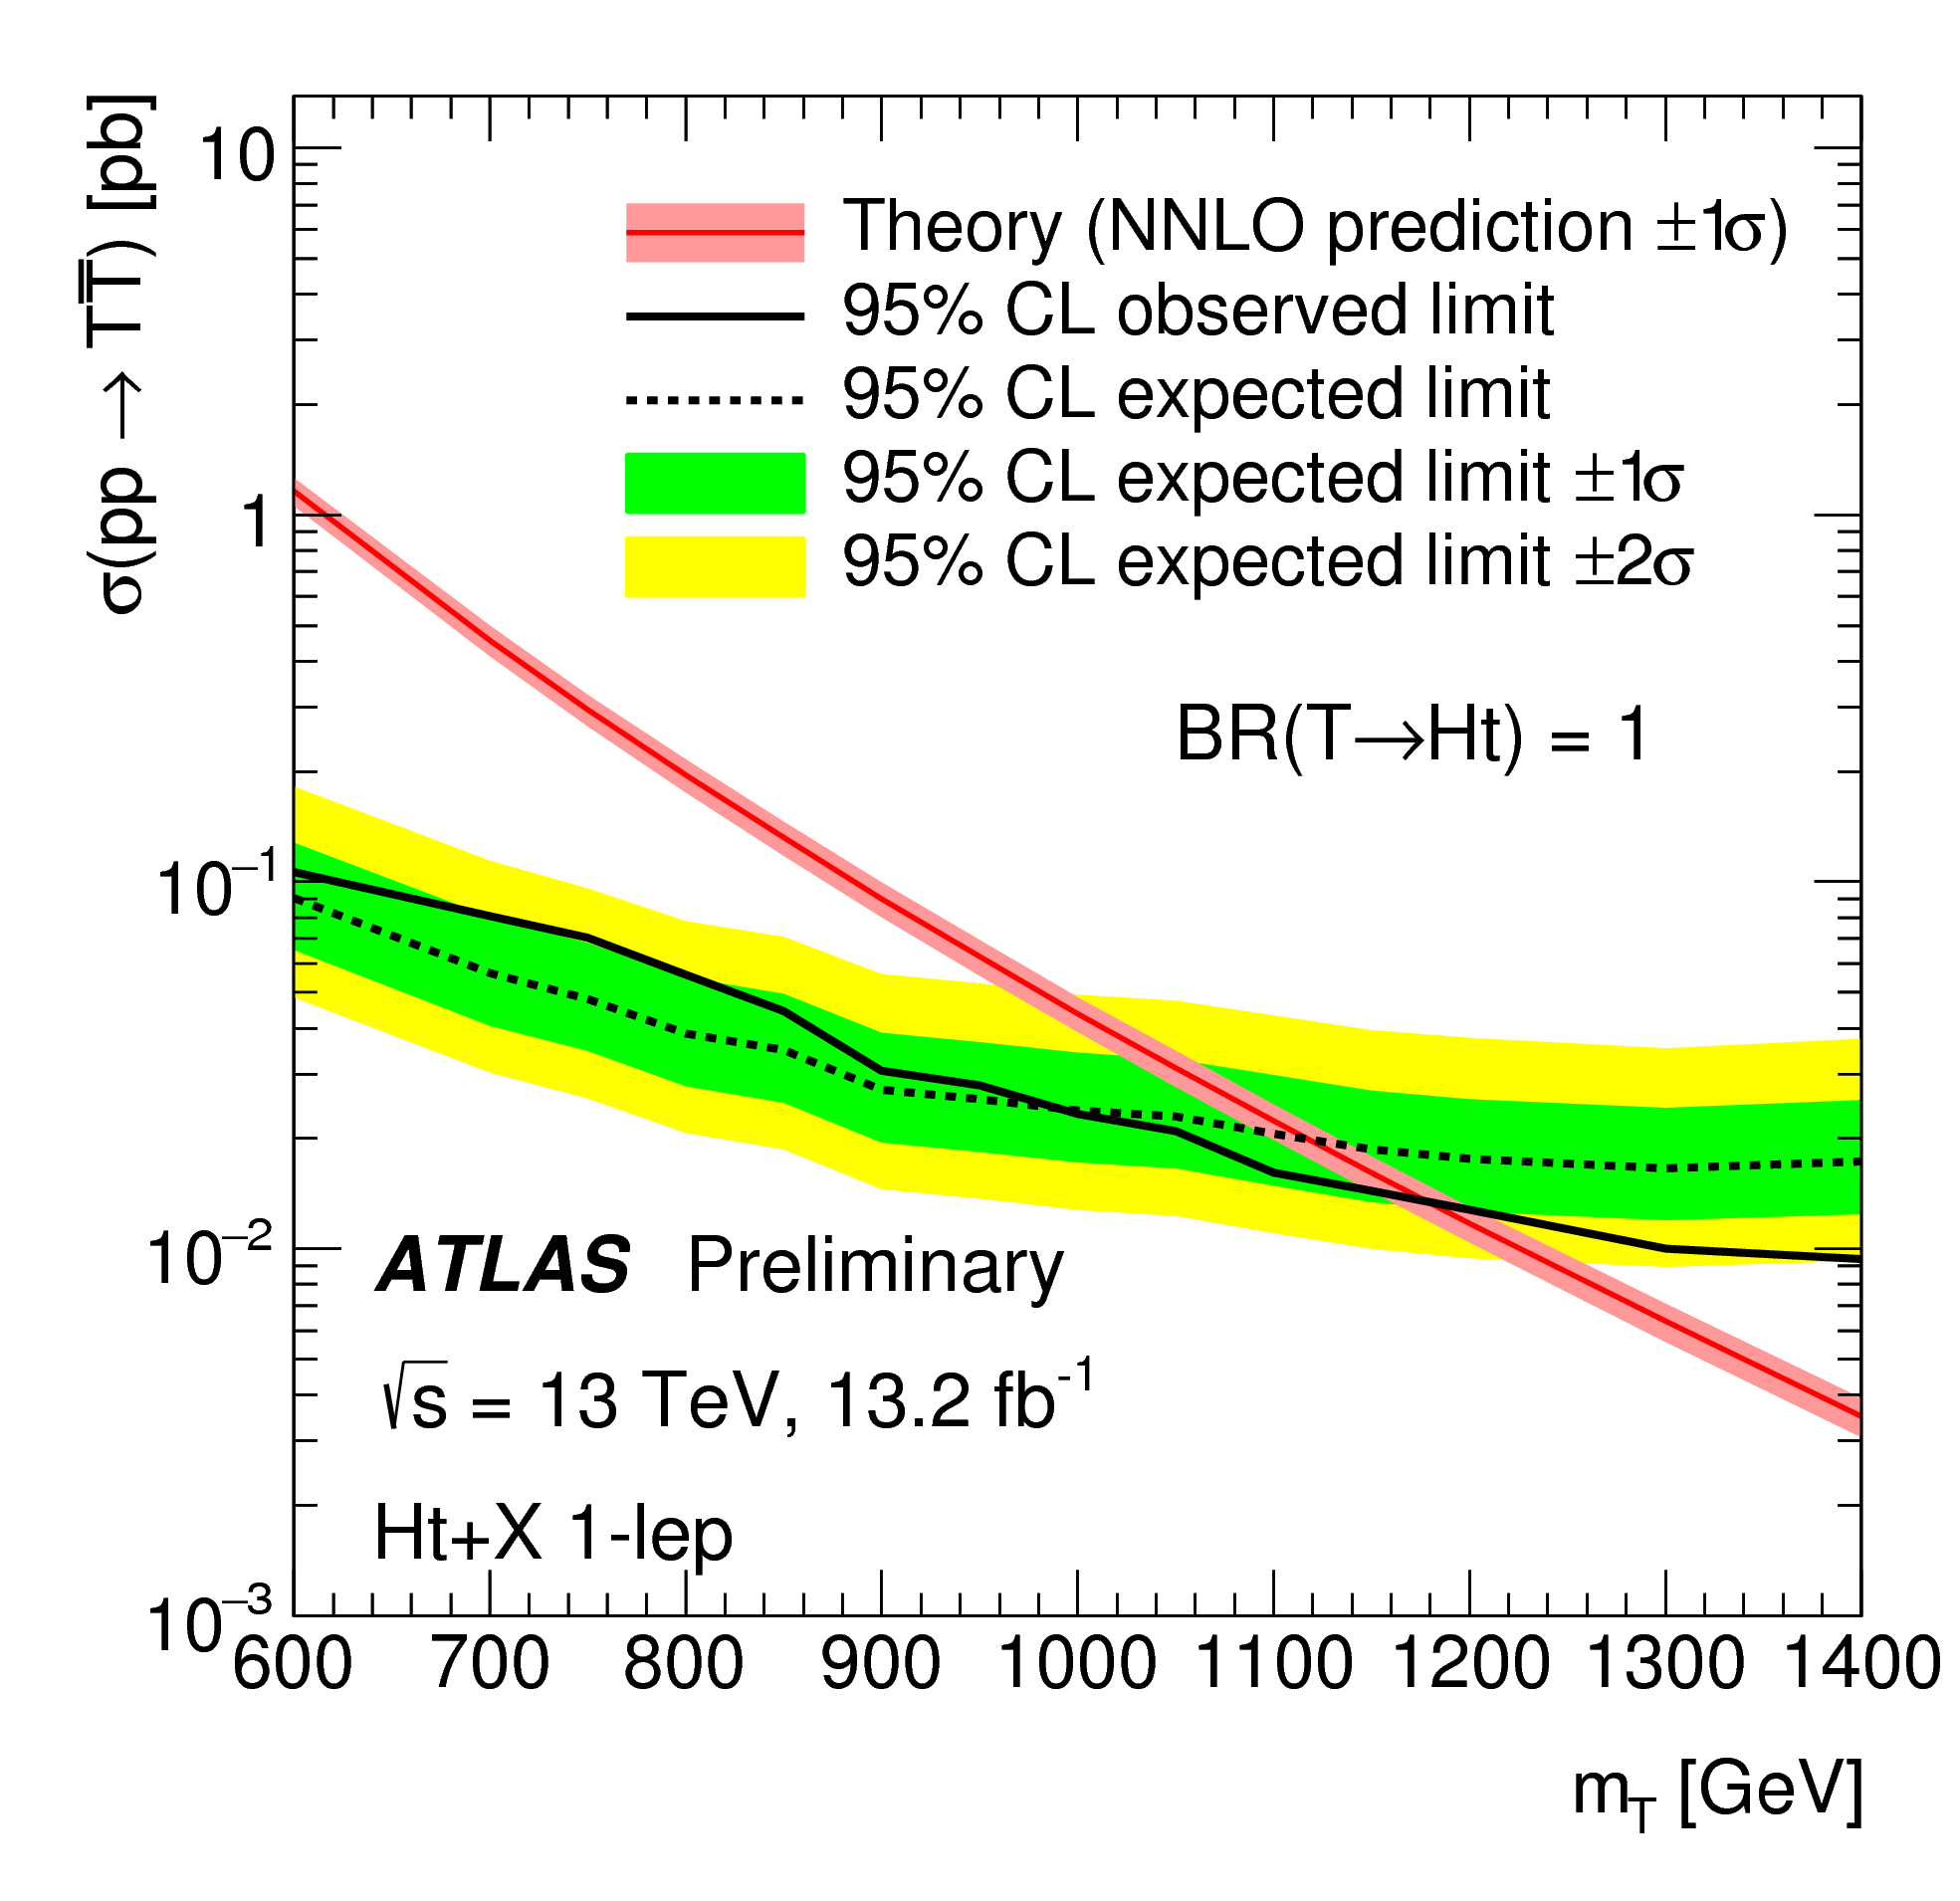
\includegraphics[width=0.9\textwidth]{figures/VLQ/fig_15a.png}
  \caption{}
  \label{}
\end{subfigure}
\begin{subfigure}{0.5\textwidth}
  \centering
  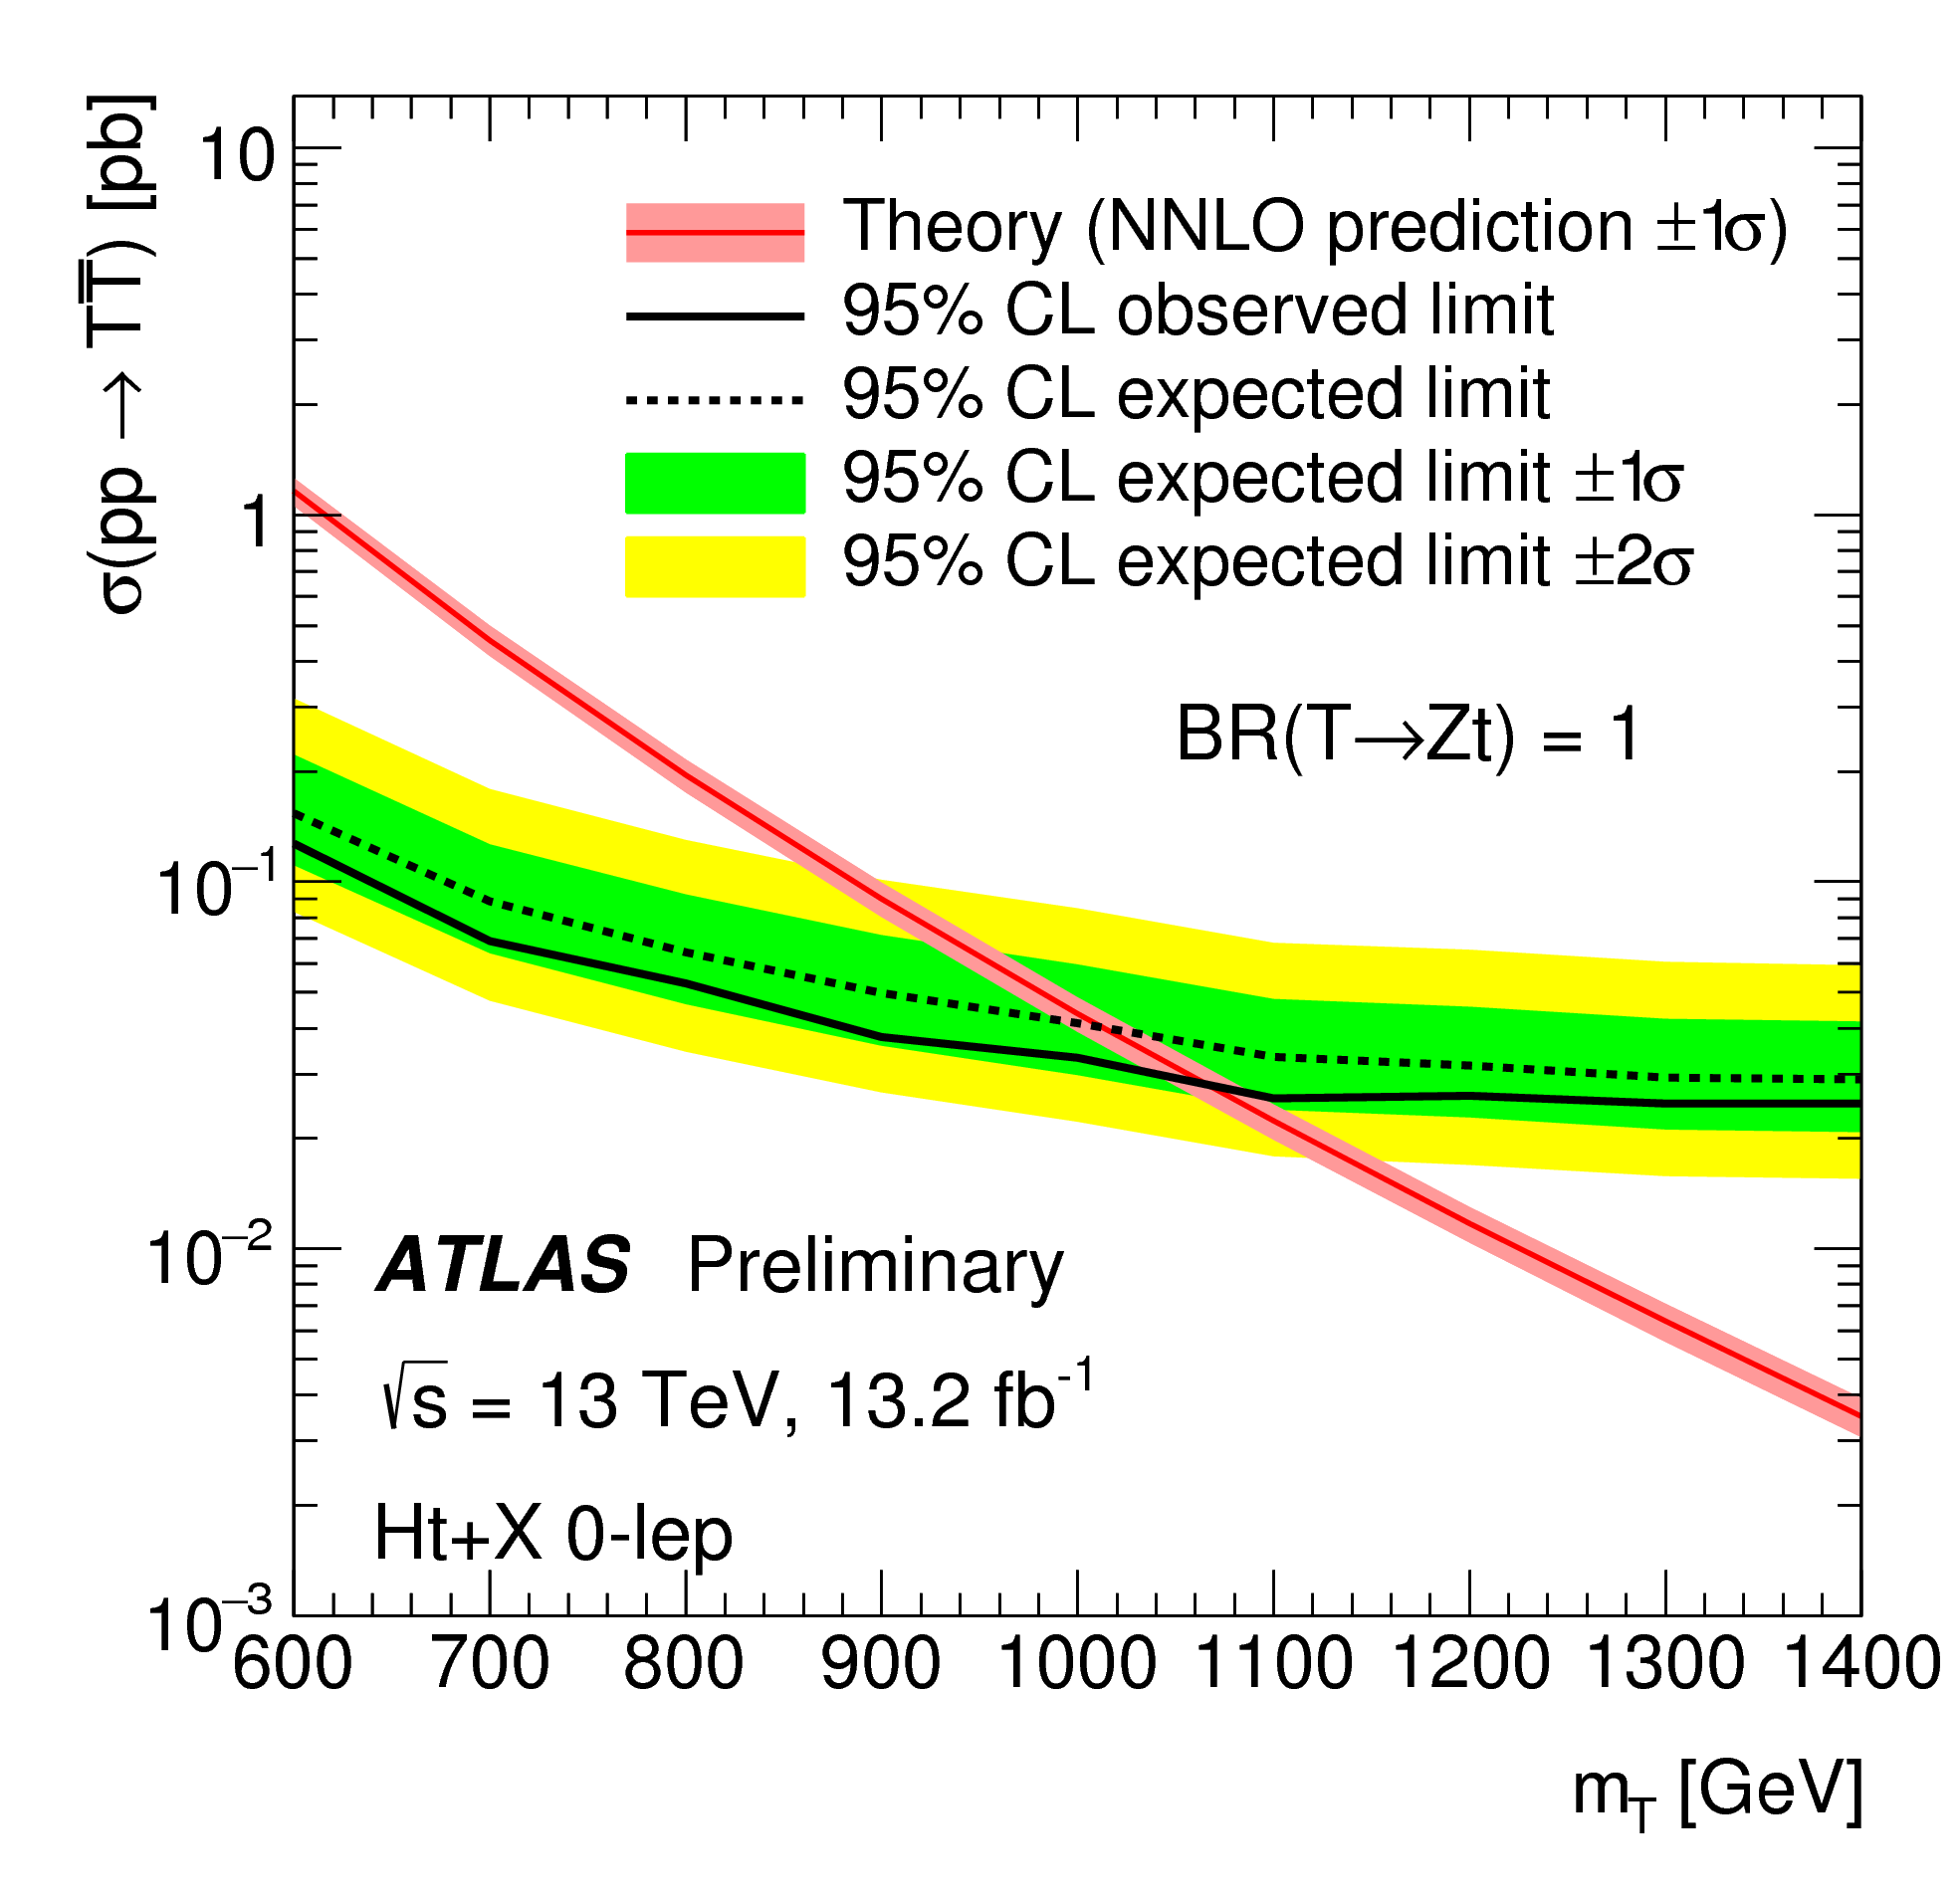
\includegraphics[width=0.9\textwidth]{figures/VLQ/fig_15b.png}
  \caption{}
  \label{}
\end{subfigure}
\captionsetup{width=0.85\textwidth} \caption{\small Observed (solid line) and expected (dashed line) 95\% CL upper limits on the $T\bar{T}$ cross section as a function of the $T$-quark mass 
for (a) the 1-lepton search under the assumption ${\rm BR}(T \to Ht)=1$, and (b) the 0-lepton search under the assumption ${\rm BR}(T \to Zt)=1$.
The surrounding shaded bands correspond to $\pm1$ and $\pm2$ standard deviations around the expected limit. 
The thin red line and band show the theoretical prediction and its $\pm1$ standard deviation uncertainty.}
\label{sec:vlq:fig:centlimit}
\end{figure}

\begin{figure}[h!]
\begin{subfigure}{0.5\textwidth}
  \centering
  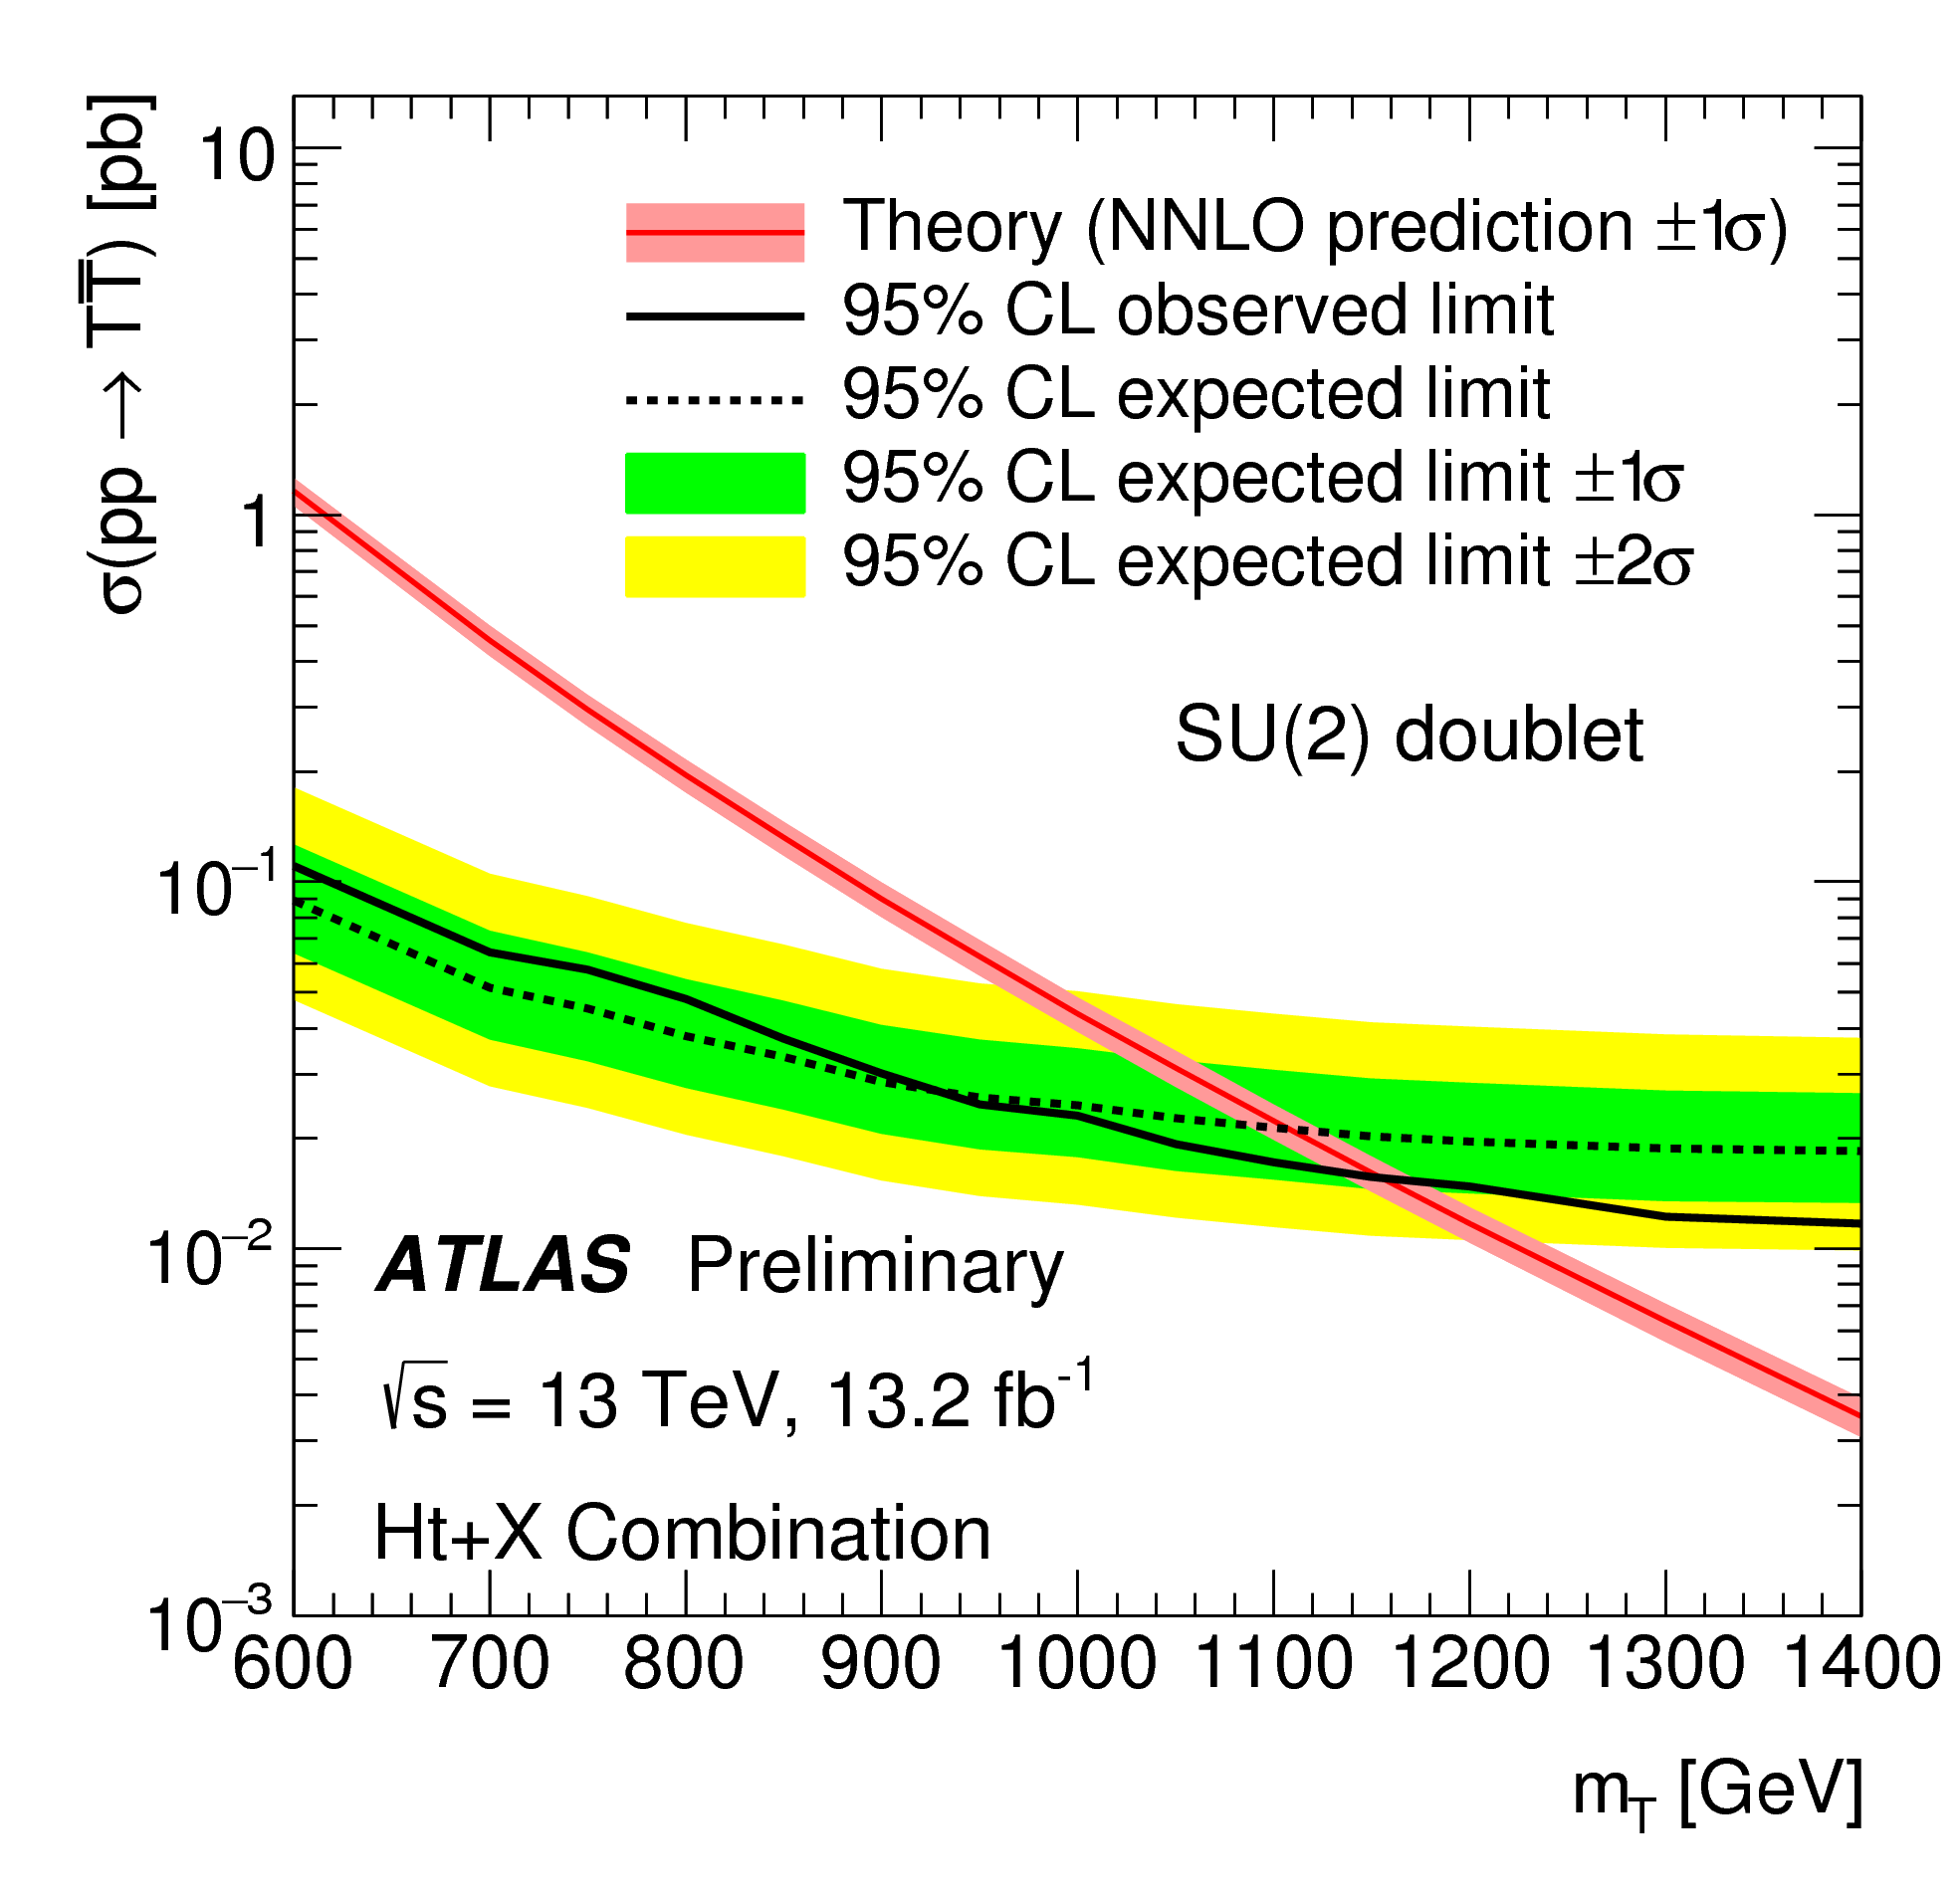
\includegraphics[width=0.9\textwidth]{figures/VLQ/fig_16a.png}
  \caption{}
  \label{}
\end{subfigure}
\begin{subfigure}{0.5\textwidth}
  \centering
  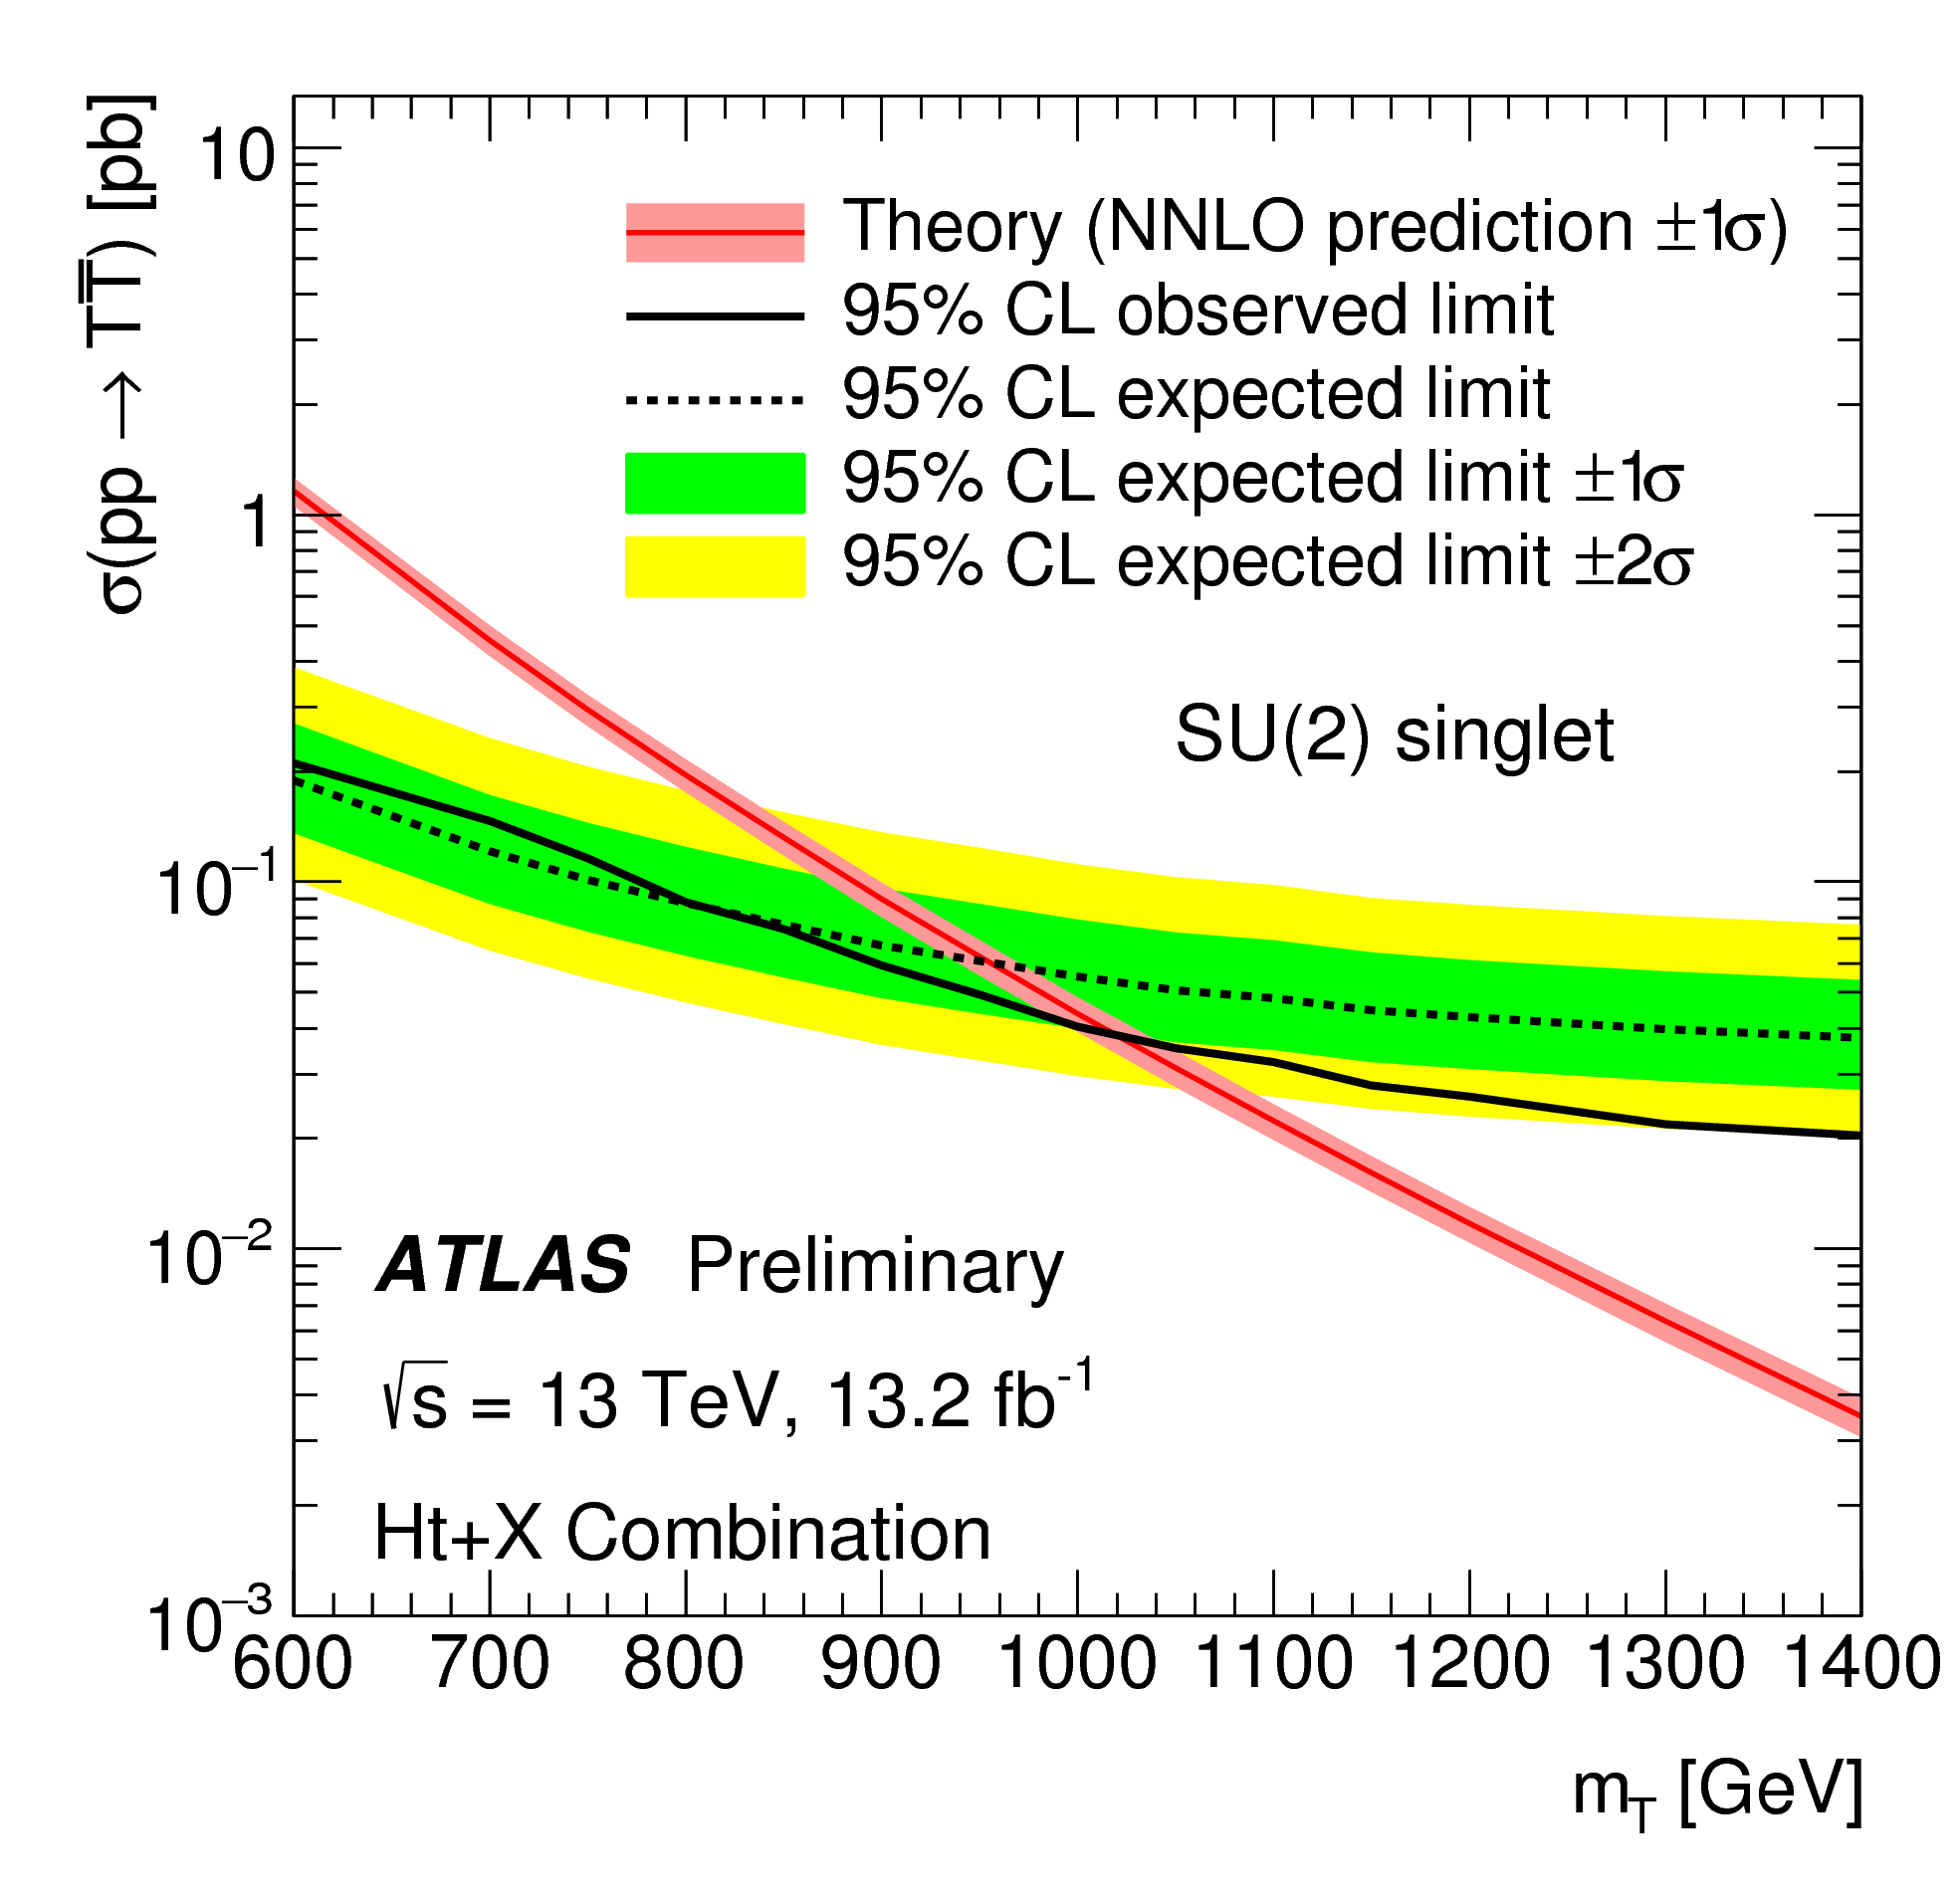
\includegraphics[width=0.9\textwidth]{figures/VLQ/fig_16b.png}
  \caption{}
  \label{}
\end{subfigure}
\captionsetup{width=0.85\textwidth} \caption{\small Observed (solid line) and expected (dashed line) 95\% CL upper limits on the $T\bar{T}$ cross section as a function of the $T$-quark mass 
for the combination of the 1-lepton and 0-lepton searches (a) for a $T$-quark doublet, and (b) for a $T$-quark singlet.
The surrounding shaded bands correspond to $\pm1$ and $\pm2$ standard deviations around the expected limit. 
The thin red line and band show the theoretical prediction and its $\pm1$ standard deviation uncertainty.}
\label{sec:vlq:fig:singdoub}
\end{figure}

For a vector-like singlet $T$-quark, an observed (expected) $95\%$ CL limit of $m_{T} > 1020$ (960) $\gev$ is obtained. For a vector-like doublet $T$-quark the observed (expected) $95\%$ CL lower limit is $m_{T} > 1160$ (1110) \gev. This is the most sensitive search to date for a vector-like top partner in the singlet and doublet scenarios.  A summary of the observed and expected upper limits on the $T$-quark mass in the different benchmark scenarios is given in table \ref{chp:vlq:tab:masslimits}, including a comparison to the limits obtained by previous $T\bar{T} \to Ht+X$ searches in the 1-lepton channel. As can be appreciated, the current results extend the sensitivity of previous searches by $\sim200-300$ \gev, depending on the assumed benchmark scenario.


\begin{table}[h!]
\begin{center}
\begin{tabular}{lccccc}
\toprule\toprule
\multicolumn{6}{c}{95\% CL lower limits on $T$-quark mass [\gev]} \\      
\midrule
%\midrule
Search & ${\rm BR}(T \to Ht)=1$ &  ${\rm BR}(T \to Zt)=1$ & Doublet & Singlet & \\
\midrule
1-lepton channel & $1180\,(1120)$ & $740\,(820)$ & $1060\,(1000)$ & $900\,(880)$ & \\
0-lepton channel &  $1090\,(1070)$ & $1060\,(1010)$ & $1090\,(1060)$ & $950\,(890)$ & \\ 
\midrule
\textbf{Combination} & $\mathbf{1200\,(1160)}$  & $\mathbf{1100\,(1040)}$ & $\mathbf{1160\,(1110)}$ & $\mathbf{1020\,(960)}$ & \\
\bottomrule
%\bottomrule
\\
\toprule
%\toprule
\multicolumn{5}{l}{Previous ATLAS $T\bar{T}\to Ht$+X searches (1-lepton) } & Ref. \\
\midrule
Run 2 (3.2 fb$^{-1}$) & $900\,(980)$ & $700\,(740)$ & $800\,(900)$ & $750\,(780)$ & \cite{ATLAS-CONF-2016-013}
 \\
Run 1  & $950\,(880)$ & $750\,(690)$ & $860\,(820)$ & $760\,(720)$ & \cite{Aad:2015kqa} 
\\
\bottomrule\bottomrule
\end{tabular}
\captionsetup{width=0.85\textwidth} \caption{\small{Summary of observed (expected) 95\% CL lower limits on $T$-quark mass (in $\gev$) for the 1-lepton and 0-lepton channels, as well as their combination,
under different assumptions on the decay branching ratios. Also shown are the corresponding limits obtained by previous ATLAS $T\bar{T}\to Ht$+X searches in the 1-lepton channel \cite{Aad:2015kqa,ATLAS-CONF-2016-013}.}}
\label{chp:vlq:tab:masslimits}
\end{center}
\end{table}


Relaxing the assumption of a fixed branching ratio, exclusion limits can be set on vector-like $T$-quark production for different values of $m_{T}$ and as a function of the two branching ratios ${\rm BR}(T \to Wb)$ and ${\rm BR}(T \to Ht)$.\footnote{The branching ratio $T \to Zt$ is determined as: ${\rm BR}(T \to Zt) = 1- {\rm BR}(T \to  Wb)-{\rm BR}(T \to Ht)$.} The resulting $95\%$ CL exclusion limits are shown in figure \ref{sec:vlq:fig:comb}, for different values of $m_{T}$ for the combination and the individual 1-lepton and 0-lepton channels. 
\begin{figure}[h!]
\centering
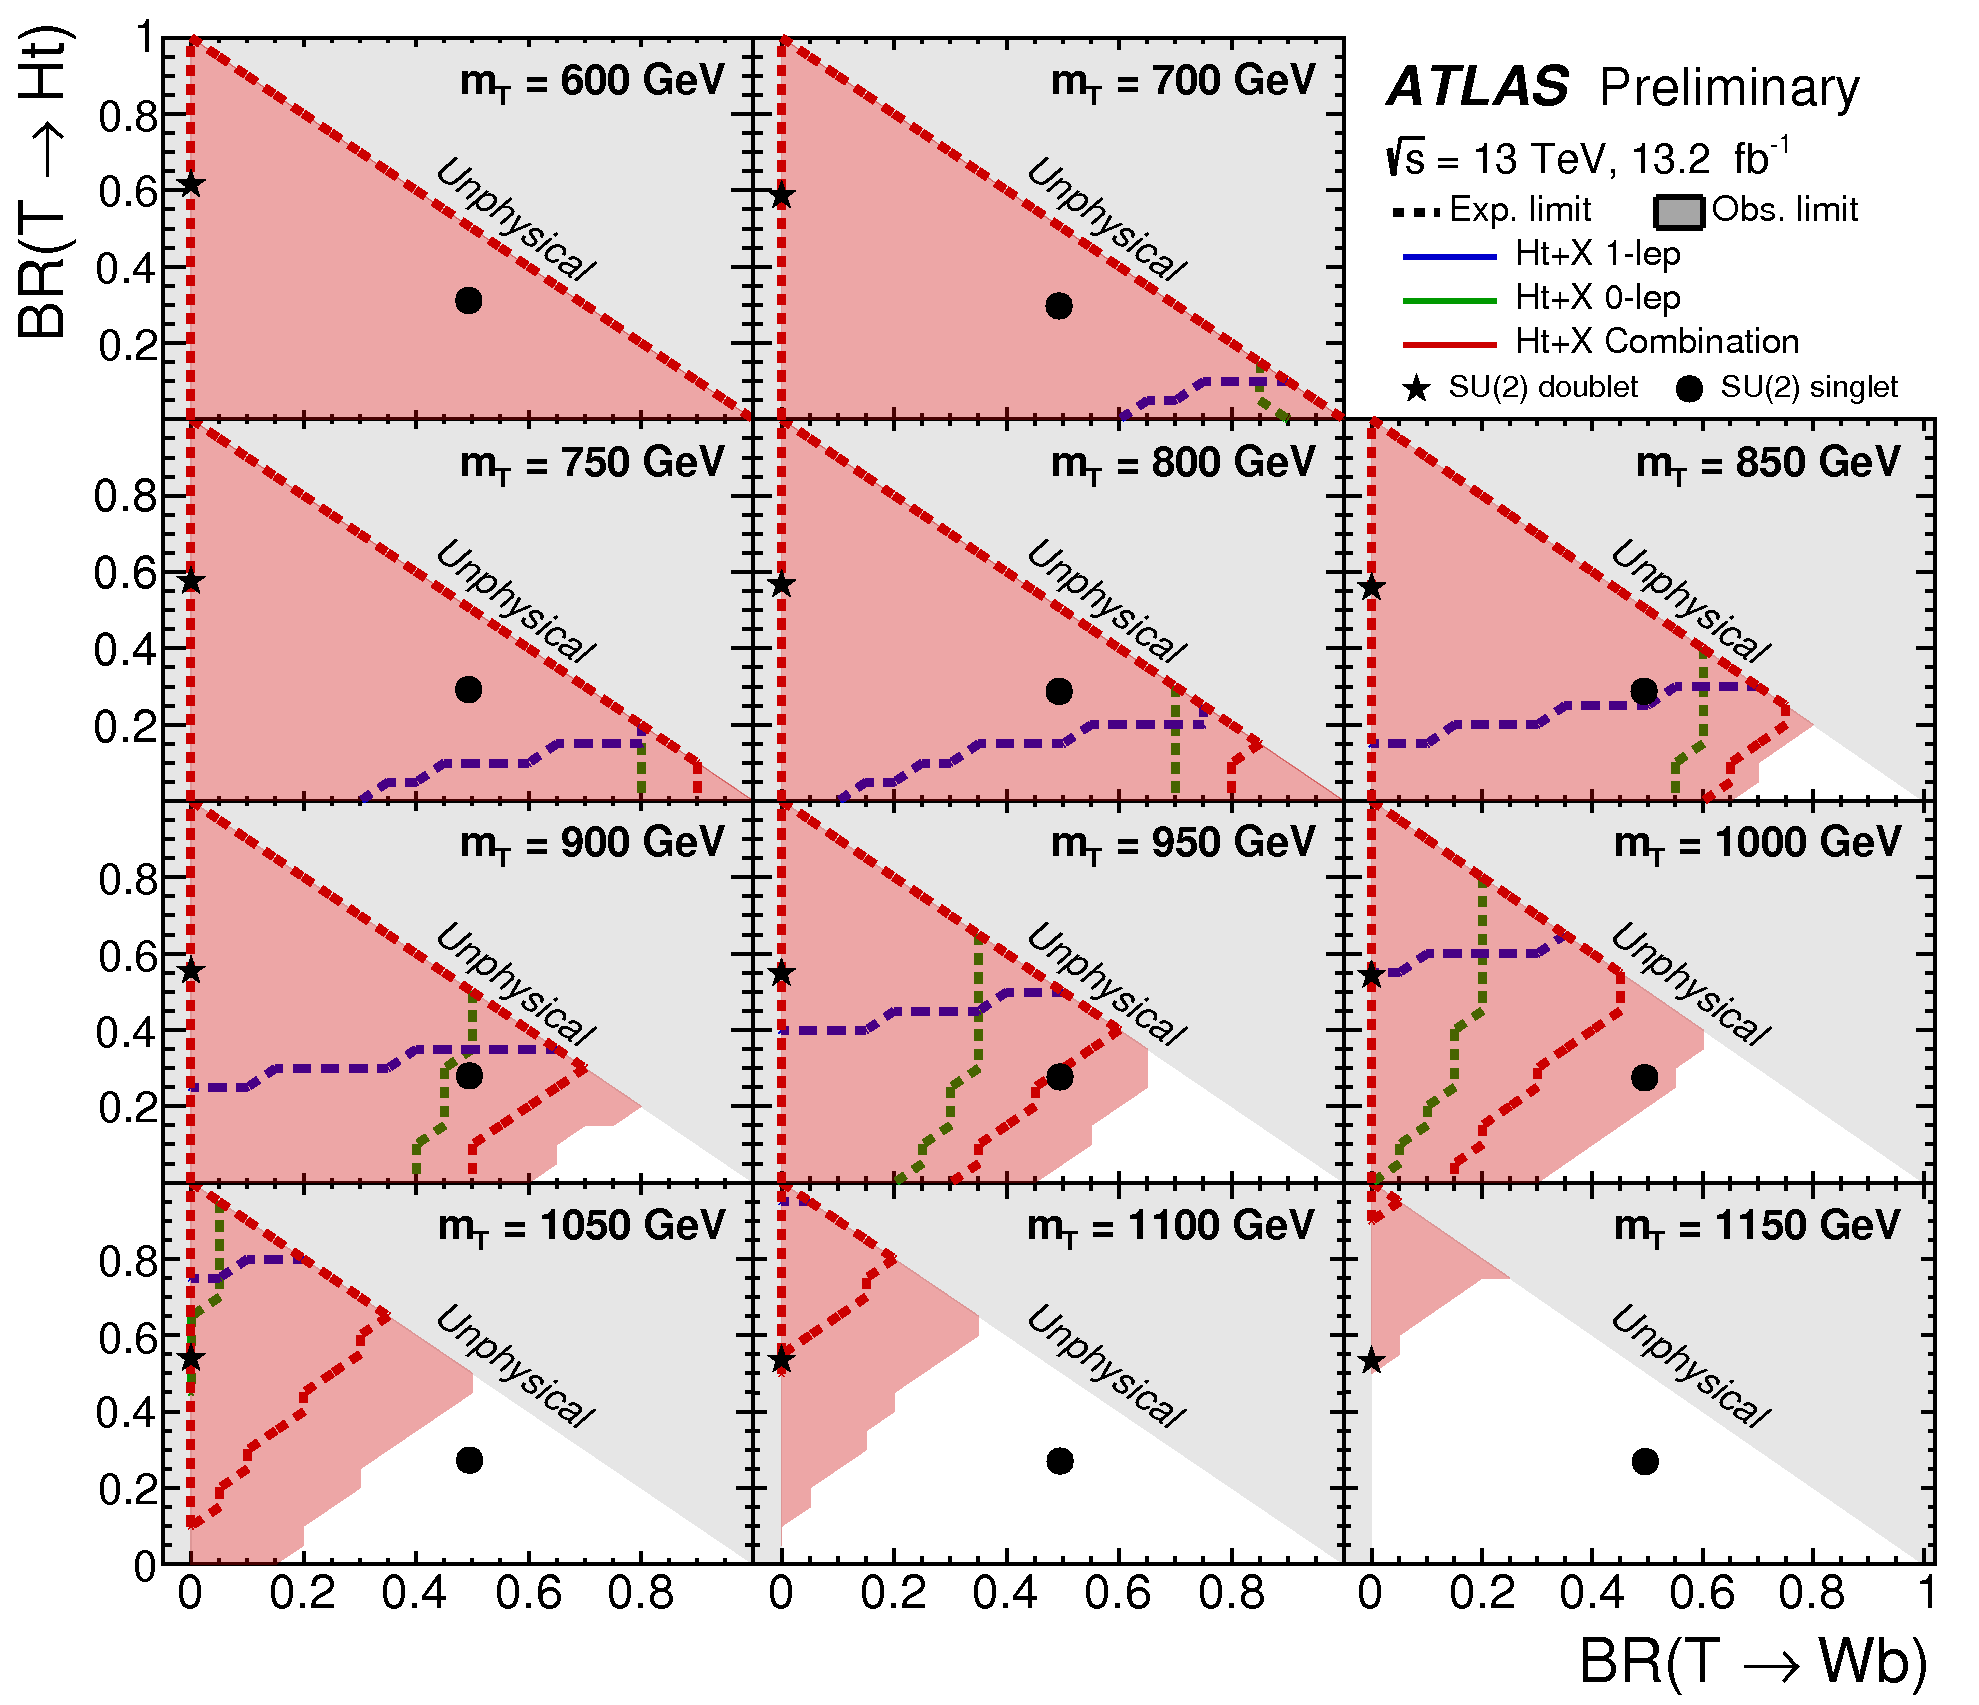
\includegraphics[width=0.8\textwidth]{figures/VLQ/fig_18.png}
 \captionsetup{width=0.85\textwidth} \caption{\small Observed (red filled area) and expected (red dashed line) $95\%$ CL exclusion in the plane of
${\rm BR}(T \to Wb)$ versus ${\rm BR}(T \to Ht)$, for different values of the vector-like $T$-quark mass for the combination of the 1-lepton and 0-lepton searches.
Also shown are the expected exclusions by the individual searches, which can be compared to that obtained through their combination.
The grey (light shaded) area corresponds to the unphysical region where the sum of branching ratios exceeds unity, or is smaller than zero.
The default branching ratio values from the {\sc Protos} event generator for the weak-isospin singlet and doublet cases 
are shown as plain circle and star symbols respectively.}
\label{sec:vlq:fig:comb}
\end{figure}
It can be noticed the complementarity between the 1-lepton and 0-lepton channels in terms of the coverage of the branching ratio plane. Therefore, the combination represents a significant improvement over the individual results. Figure \ref{sec:vlq:fig:tempplot} presents the corresponding observed and expected $T$-quark mass limits in the plane of ${\rm BR}(T \to Ht)$ versus ${\rm BR}(T \to Wb)$ for the combination obtained by linear interpolation of the calculated CL$_s$ versus $m_{T}$. The result is an observed lower limit on the $T$-quark mass ranging between 810 $\gev$ and 1200 $\gev$ for all possible values of the branching ratios into the three decay modes. This implies that a $T$-quark with mass below 810 $\gev$ is excluded at $95\%$ CL for any branching ratio configuration. The corresponding range of expected lower limits is between 730 $\gev$ and 1160 \gev.


\begin{figure}[h!]
\begin{subfigure}{0.5\textwidth}
  \centering
  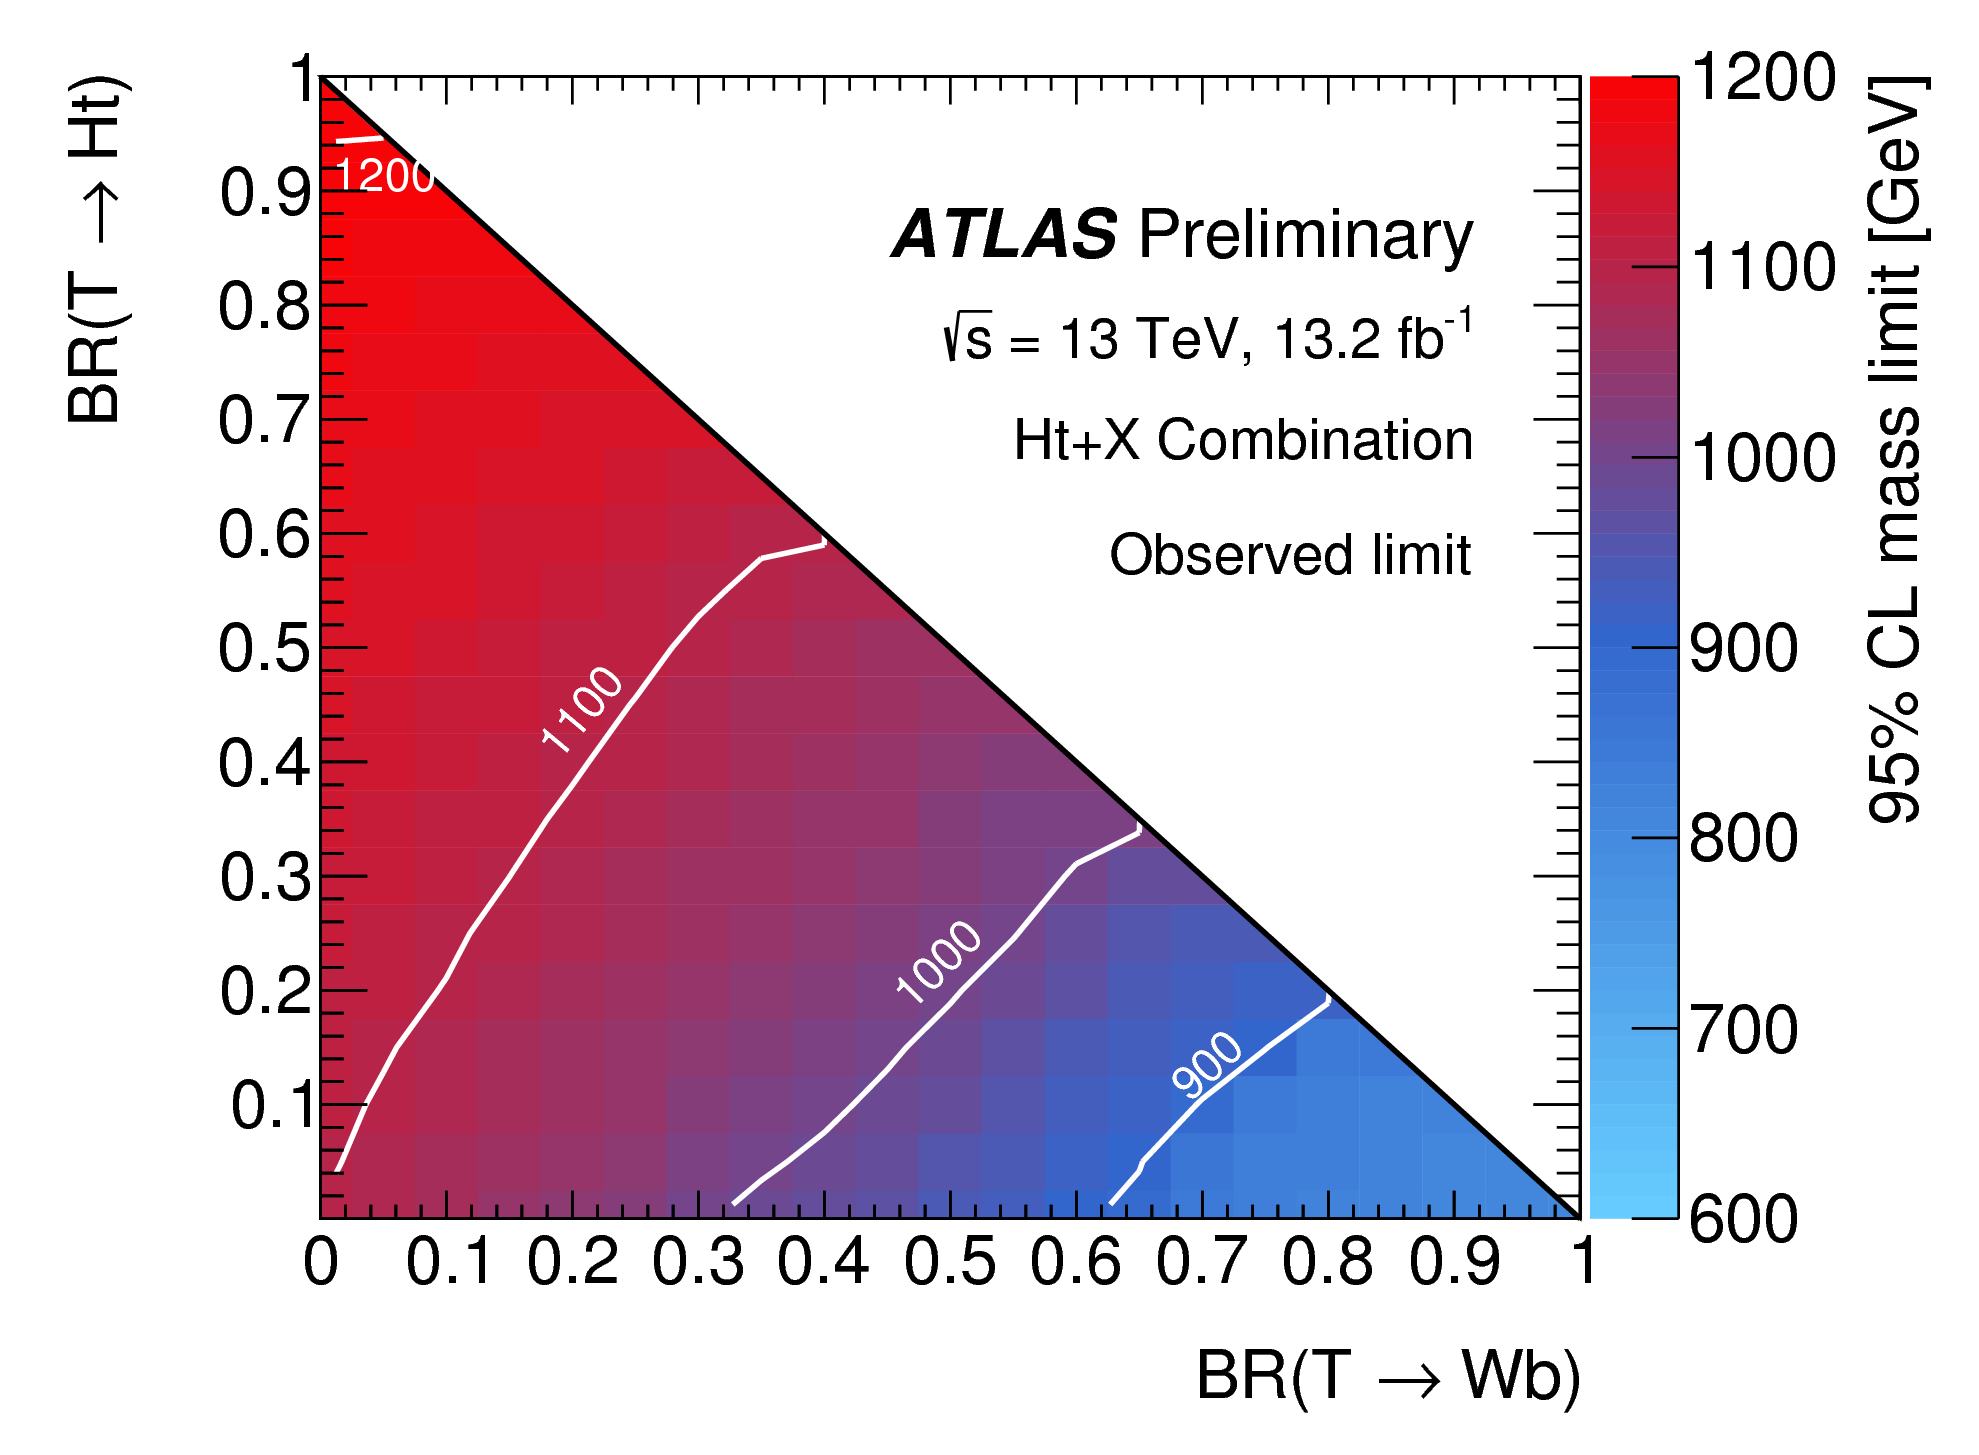
\includegraphics[width=0.9\textwidth]{figures/VLQ/fig_19a.png}
  \caption{}
  \label{}
\end{subfigure}
\begin{subfigure}{0.5\textwidth}
  \centering
  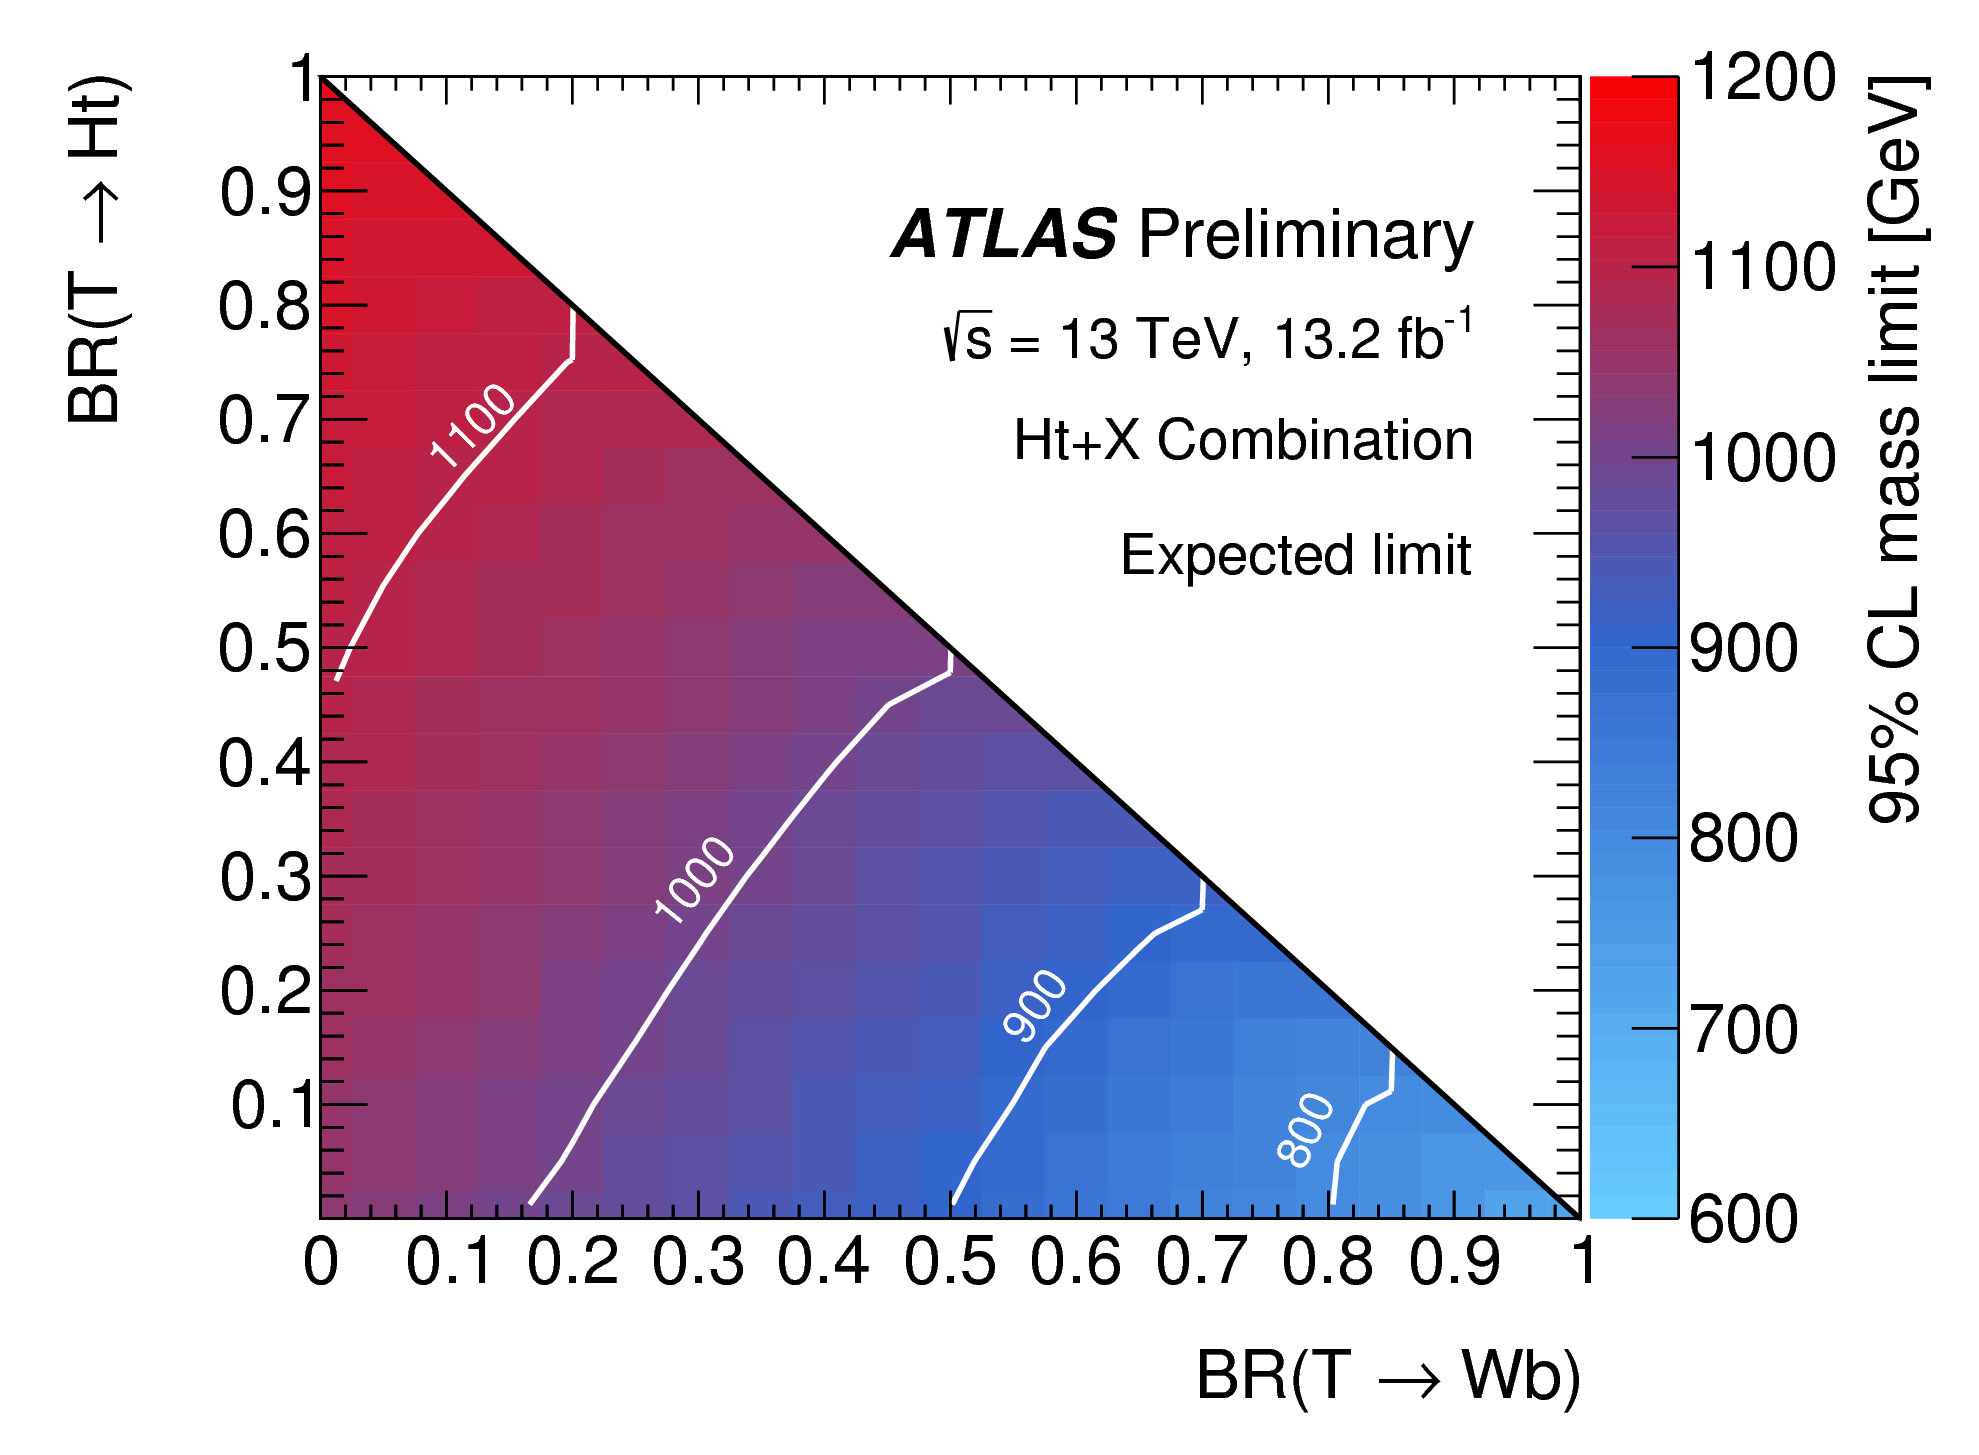
\includegraphics[width=0.9\textwidth]{figures/VLQ/fig_19b.png}
  \caption{}
  \label{}
\end{subfigure}
\captionsetup{width=0.85\textwidth} \caption{\small (a) Observed and (b) expected limit (95\% CL) on the mass of the $T$ quark in the plane 
of ${\rm BR}(T \to Ht)$ versus ${\rm BR}(T \to Wb)$ for the combination of the 1-lepton and 0-lepton searches. 
Contour lines are provided to guide the eye.}
\label{sec:vlq:fig:tempplot}
\end{figure}

\subsection{Comparison with other Run 2 searches}

In addition to the  $T\bar{T}\to Ht+X$ search, the ATLAS Collaboration has performed searches for $T\bar{T}$ production using the $\sqrt{s}=13$ $\tev$ dataset in several final states: lepton+jets final state with low jet multiplicity with low and high \MET (referred to as $Wb+X$ \cite{ATLAS-CONF-2016-102} and $Zt+X$ \cite{ATLAS-CONF-2016-101} searches respectively) and same-charge dileptons/trileptons with $b$-jets \cite{ATLAS-CONF-2016-032} (referred to as $Zb/t+X$ search). These searches have overlapping selections and thus a combination of all analyses in ATLAS has not been attempted yet. Figures \ref{sec:vlq:fig:Wb}$-$\ref{sec:vlq:fig:SS} summarise the observed and expected $T$-quark mass limits in the plane of ${\rm BR}(T \to Ht)$ versus ${\rm BR}(T \to Wb)$, set by these searches.
The $Wb+X$ and $Zt+X$ searches target respectively the $Wb$ and $Zt$ corner in the branching ratio plane and complement the coverage of the $Ht+X$ search. For example the $Ht+X$ search alone is not able to exclude at $95\%$ CL a $T$ quark with mass below 900 $\gev$ for any branching ratio configuration, but considering the $Wb+X$ and $Zt+X$ searches it can be excluded. The $Zb/t+X$ search has a similar exclusion shape in the branching ratio plane to the $Ht+X$ 0-lepton channel, but with a limited sensitivity. Therefore, to date the $Zb/t+X$ search does not add new information to the branching ratio exclusion plane.
The CMS Collaboration in Run 2 has performed a $Wb+X$ search \cite{CMS-PAS-B2G-16-002} with  observed (expected) lower limits on the $T$-quark mass ranging between $\sim700$ $\gev$ and 850 $\gev$ ($\sim700$ $\gev$ and 870 $\gev$) and a $Ht+X$ search \cite{CMS-PAS-B2G-16-011} with corresponding  observed (expected) limits ranging between $\sim700$ $\gev$ and 860 $\gev$ ($\sim700$ $\gev$ and 870 $\gev$).\\ \indent
In summary, the $Ht+X$ search presented in this dissertation is  to date the most sensitive search for the well-motivated singlet and doublet benchmarks, and the search with the widest coverage in the branching ratio plane.


\begin{figure}[h!]
\begin{subfigure}{0.5\textwidth}
  \centering
  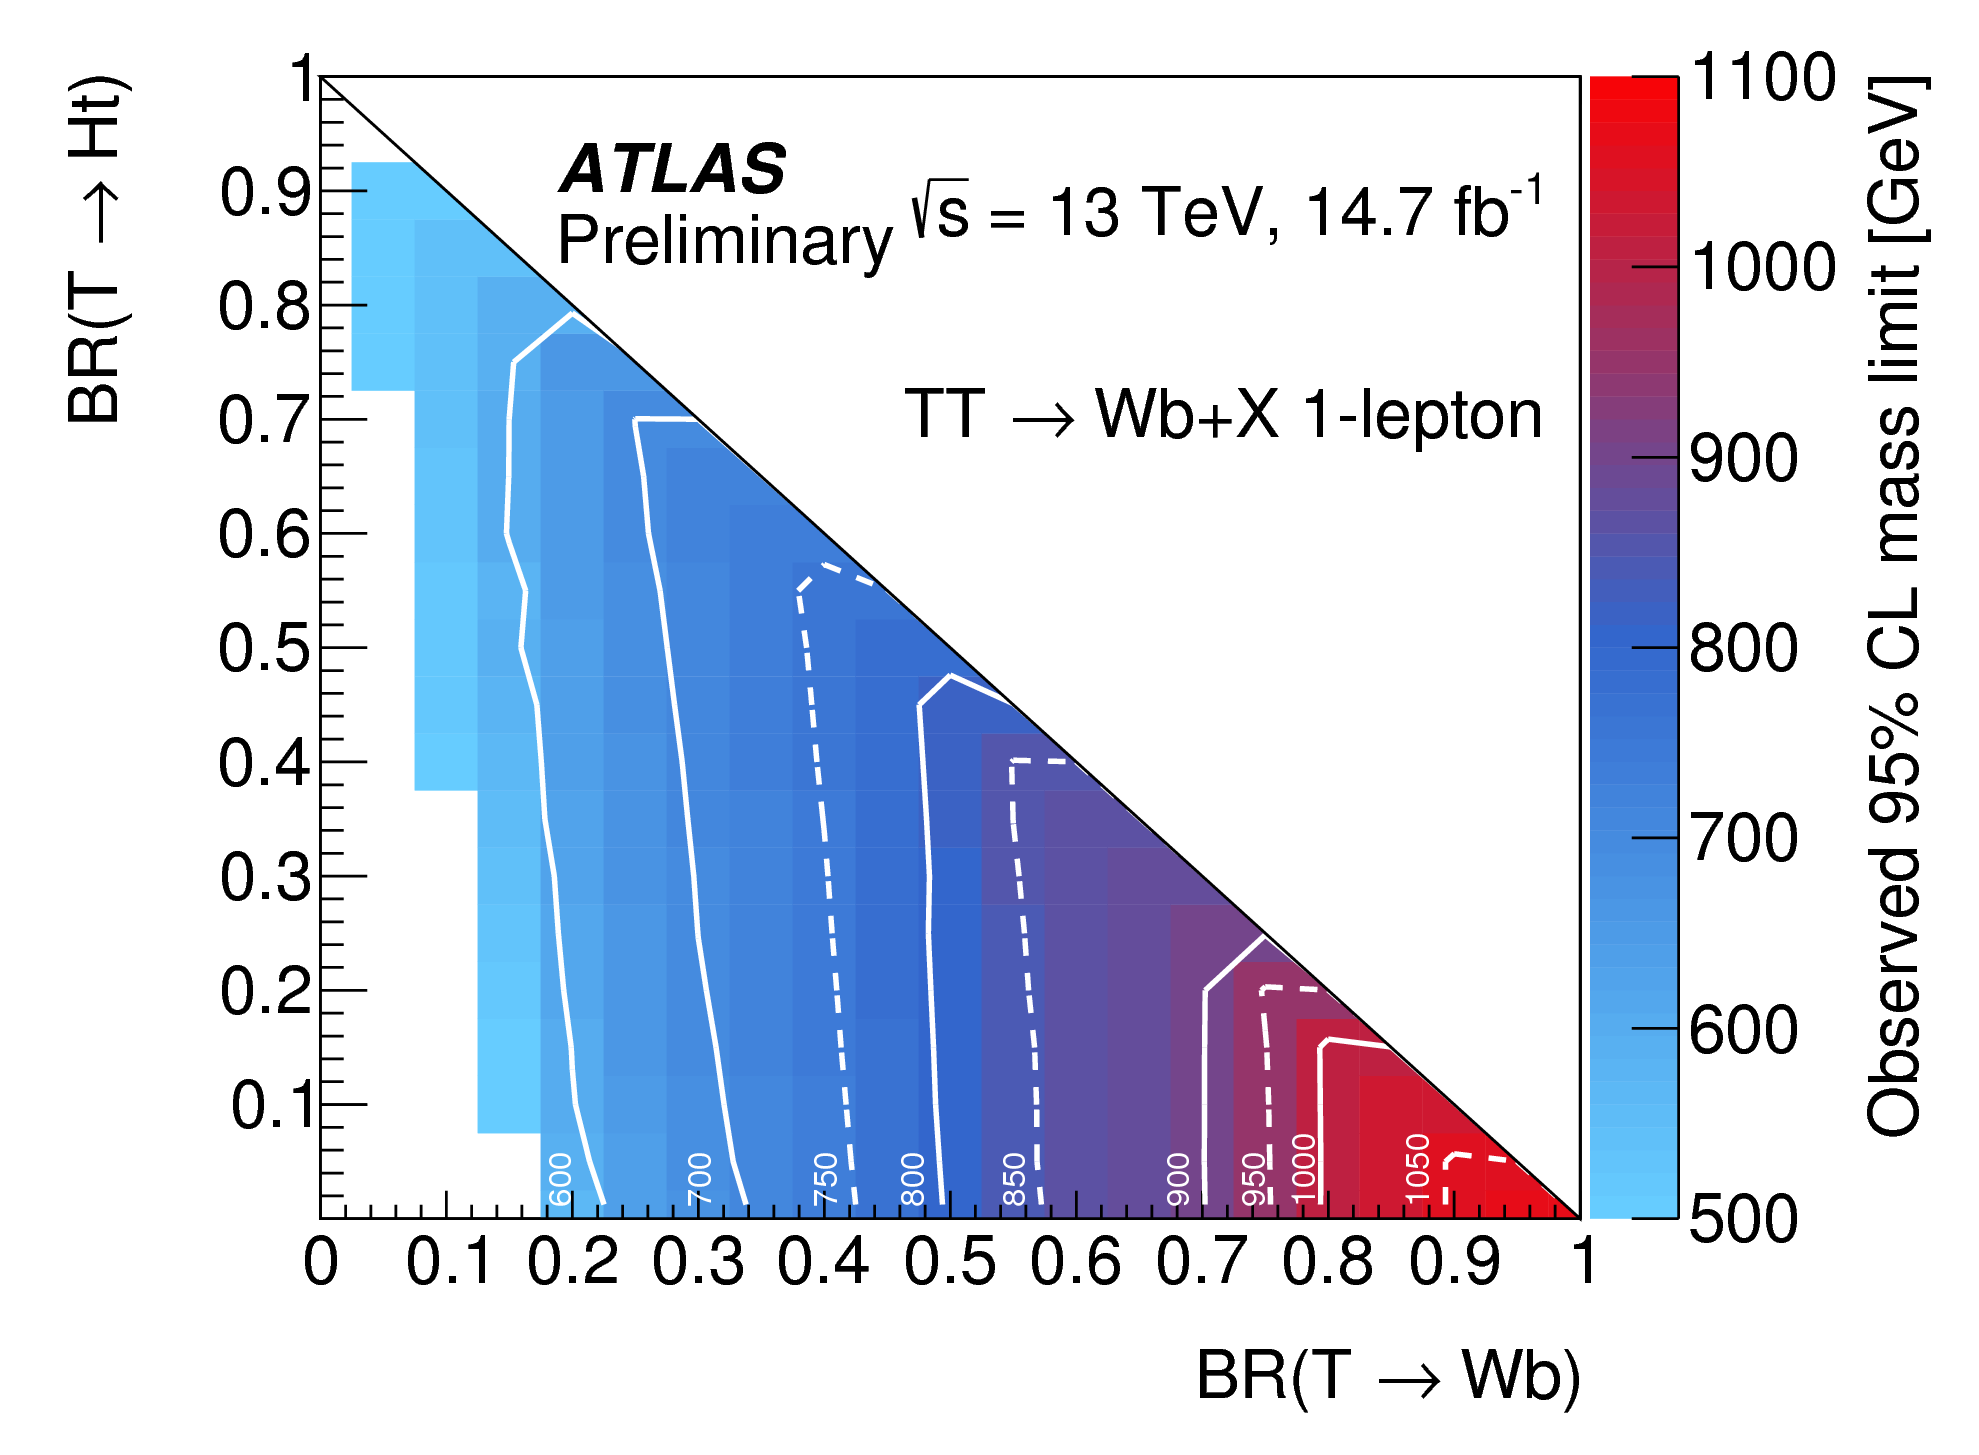
\includegraphics[width=0.9\textwidth]{figures/VLQ/Wbb.png}
  \caption{}
  \label{}
\end{subfigure}
\begin{subfigure}{0.5\textwidth}
  \centering
  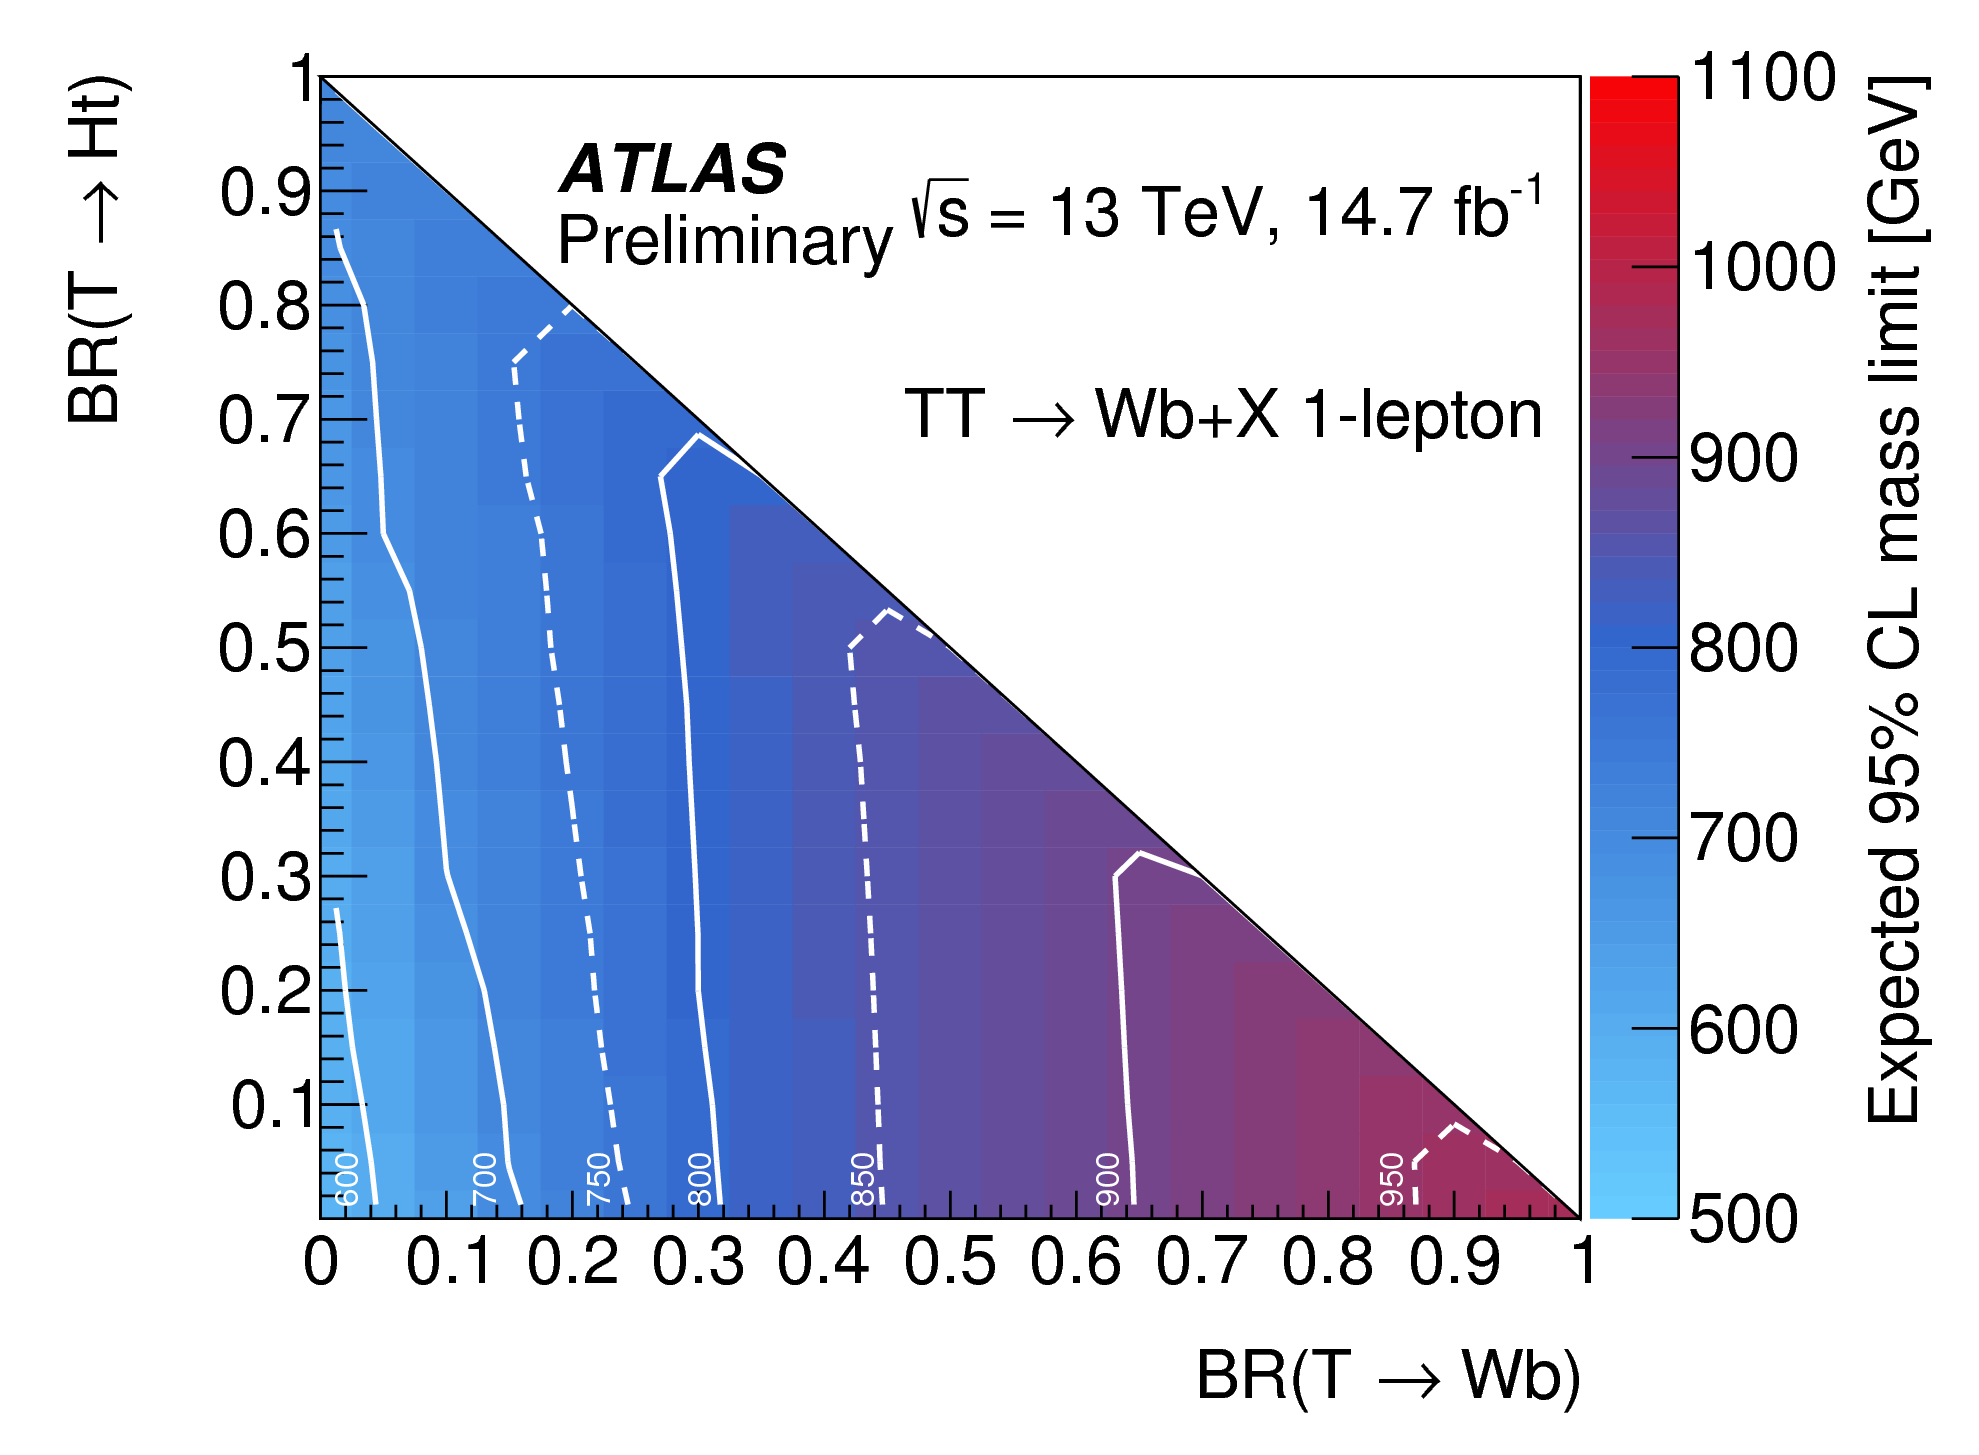
\includegraphics[width=0.9\textwidth]{figures/VLQ/Wba.png}
  \caption{}
  \label{}
\end{subfigure}
\captionsetup{width=0.85\textwidth} \caption{\small (a) Observed and (b) expected limit (95\% CL) on the mass of the $T$ quark in the plane 
of ${\rm BR}(T \to Ht)$ versus ${\rm BR}(T \to Wb)$ for the $Wb+X$ search. 
Contour lines are provided to guide the eye.}
\label{sec:vlq:fig:Wb}
\end{figure}

\begin{figure}[h!]
\begin{subfigure}{0.5\textwidth}
  \centering
  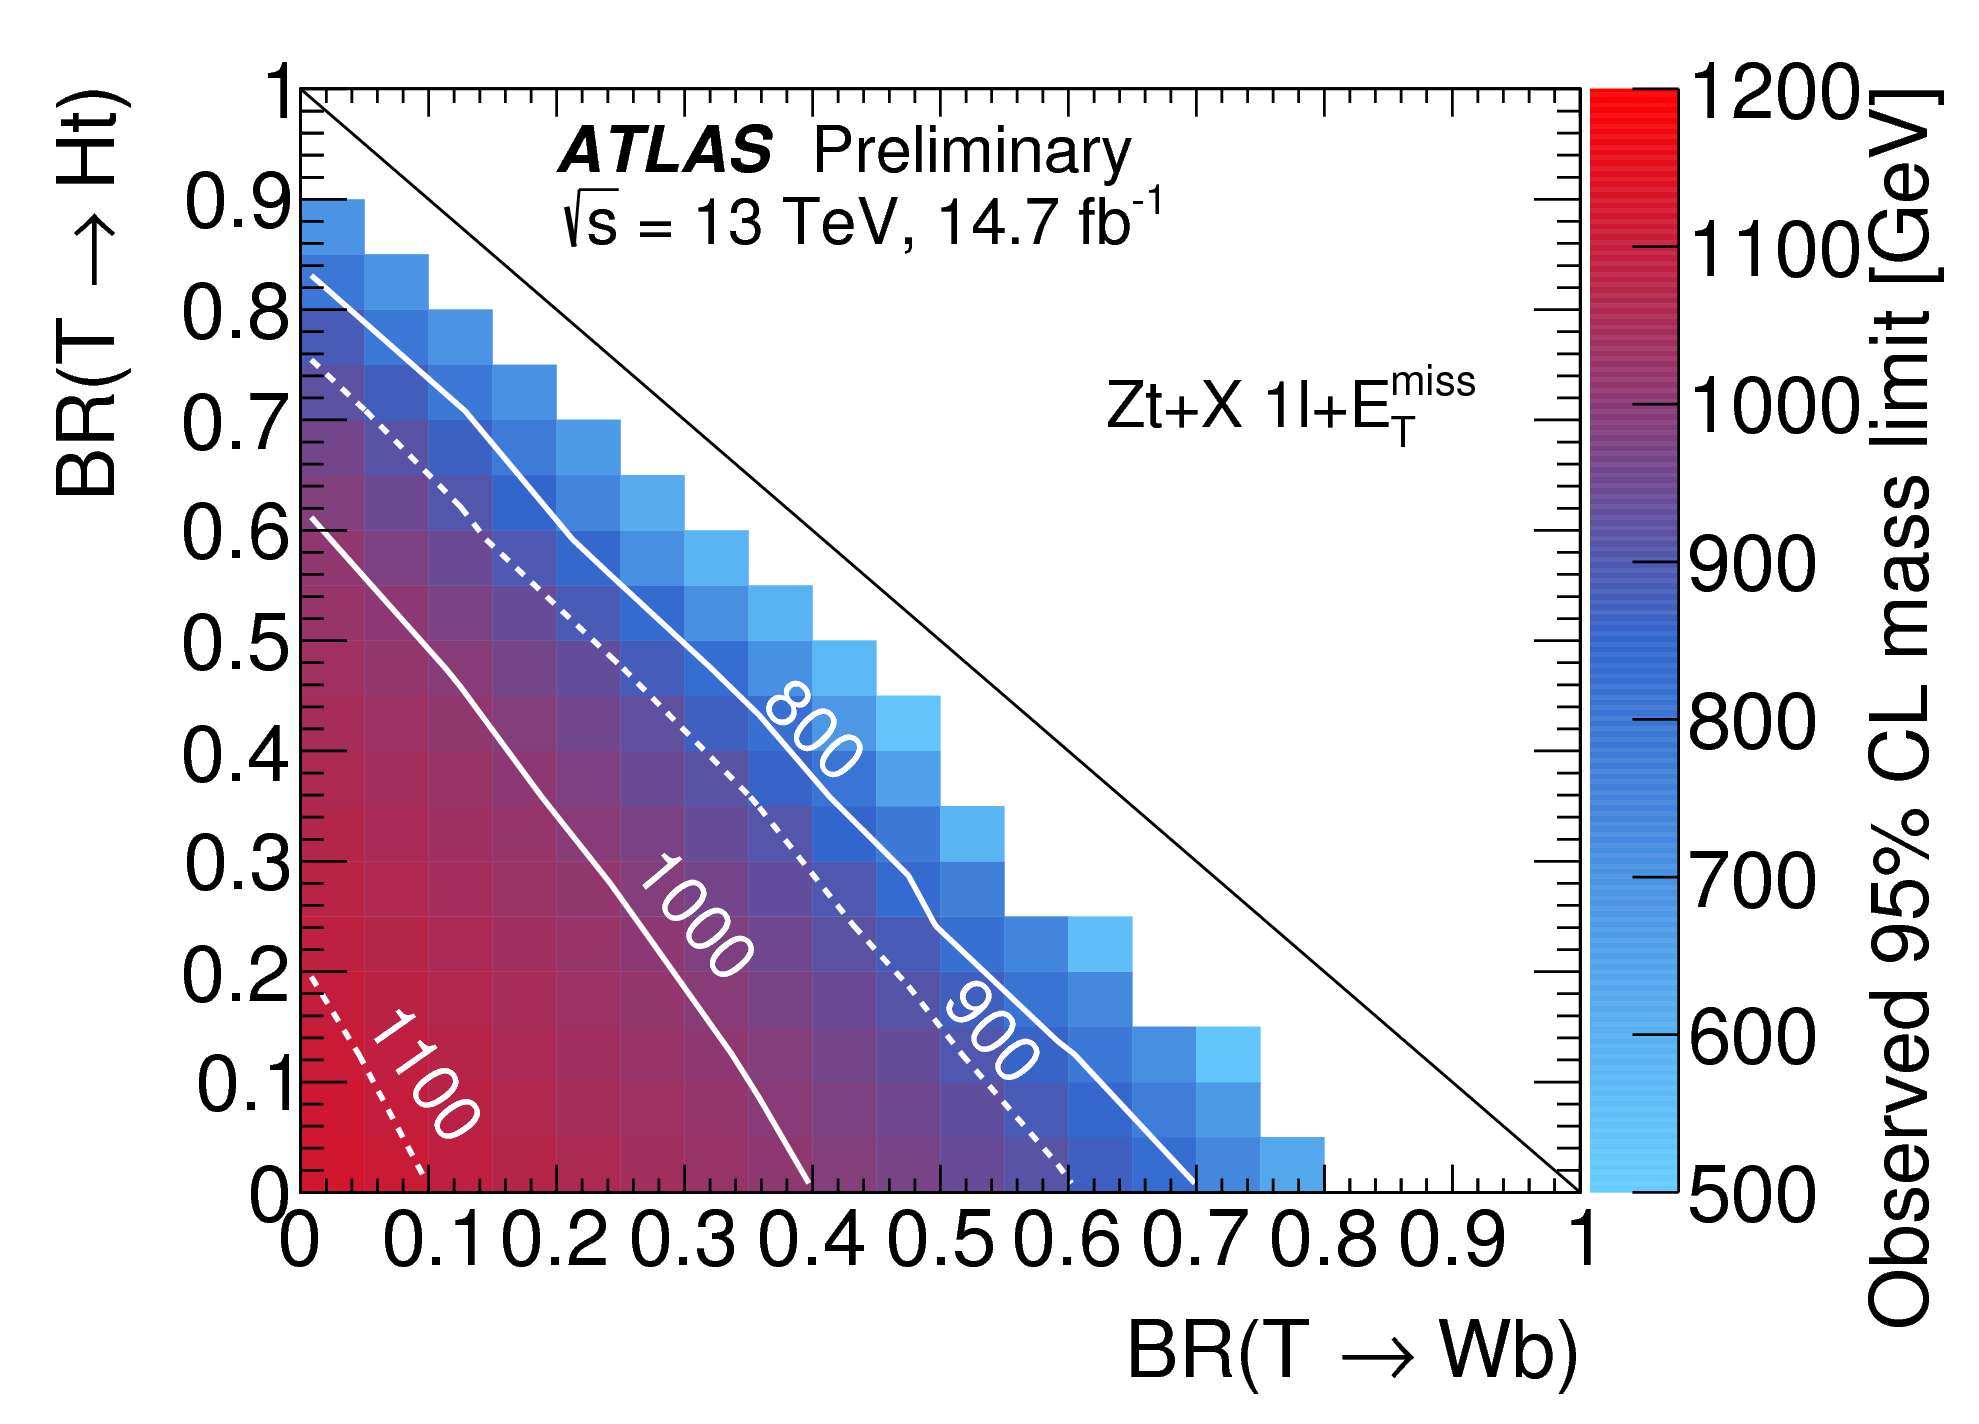
\includegraphics[width=0.9\textwidth]{figures/VLQ/Ztb.png}
  \caption{}
  \label{}
\end{subfigure}
\begin{subfigure}{0.5\textwidth}
  \centering
  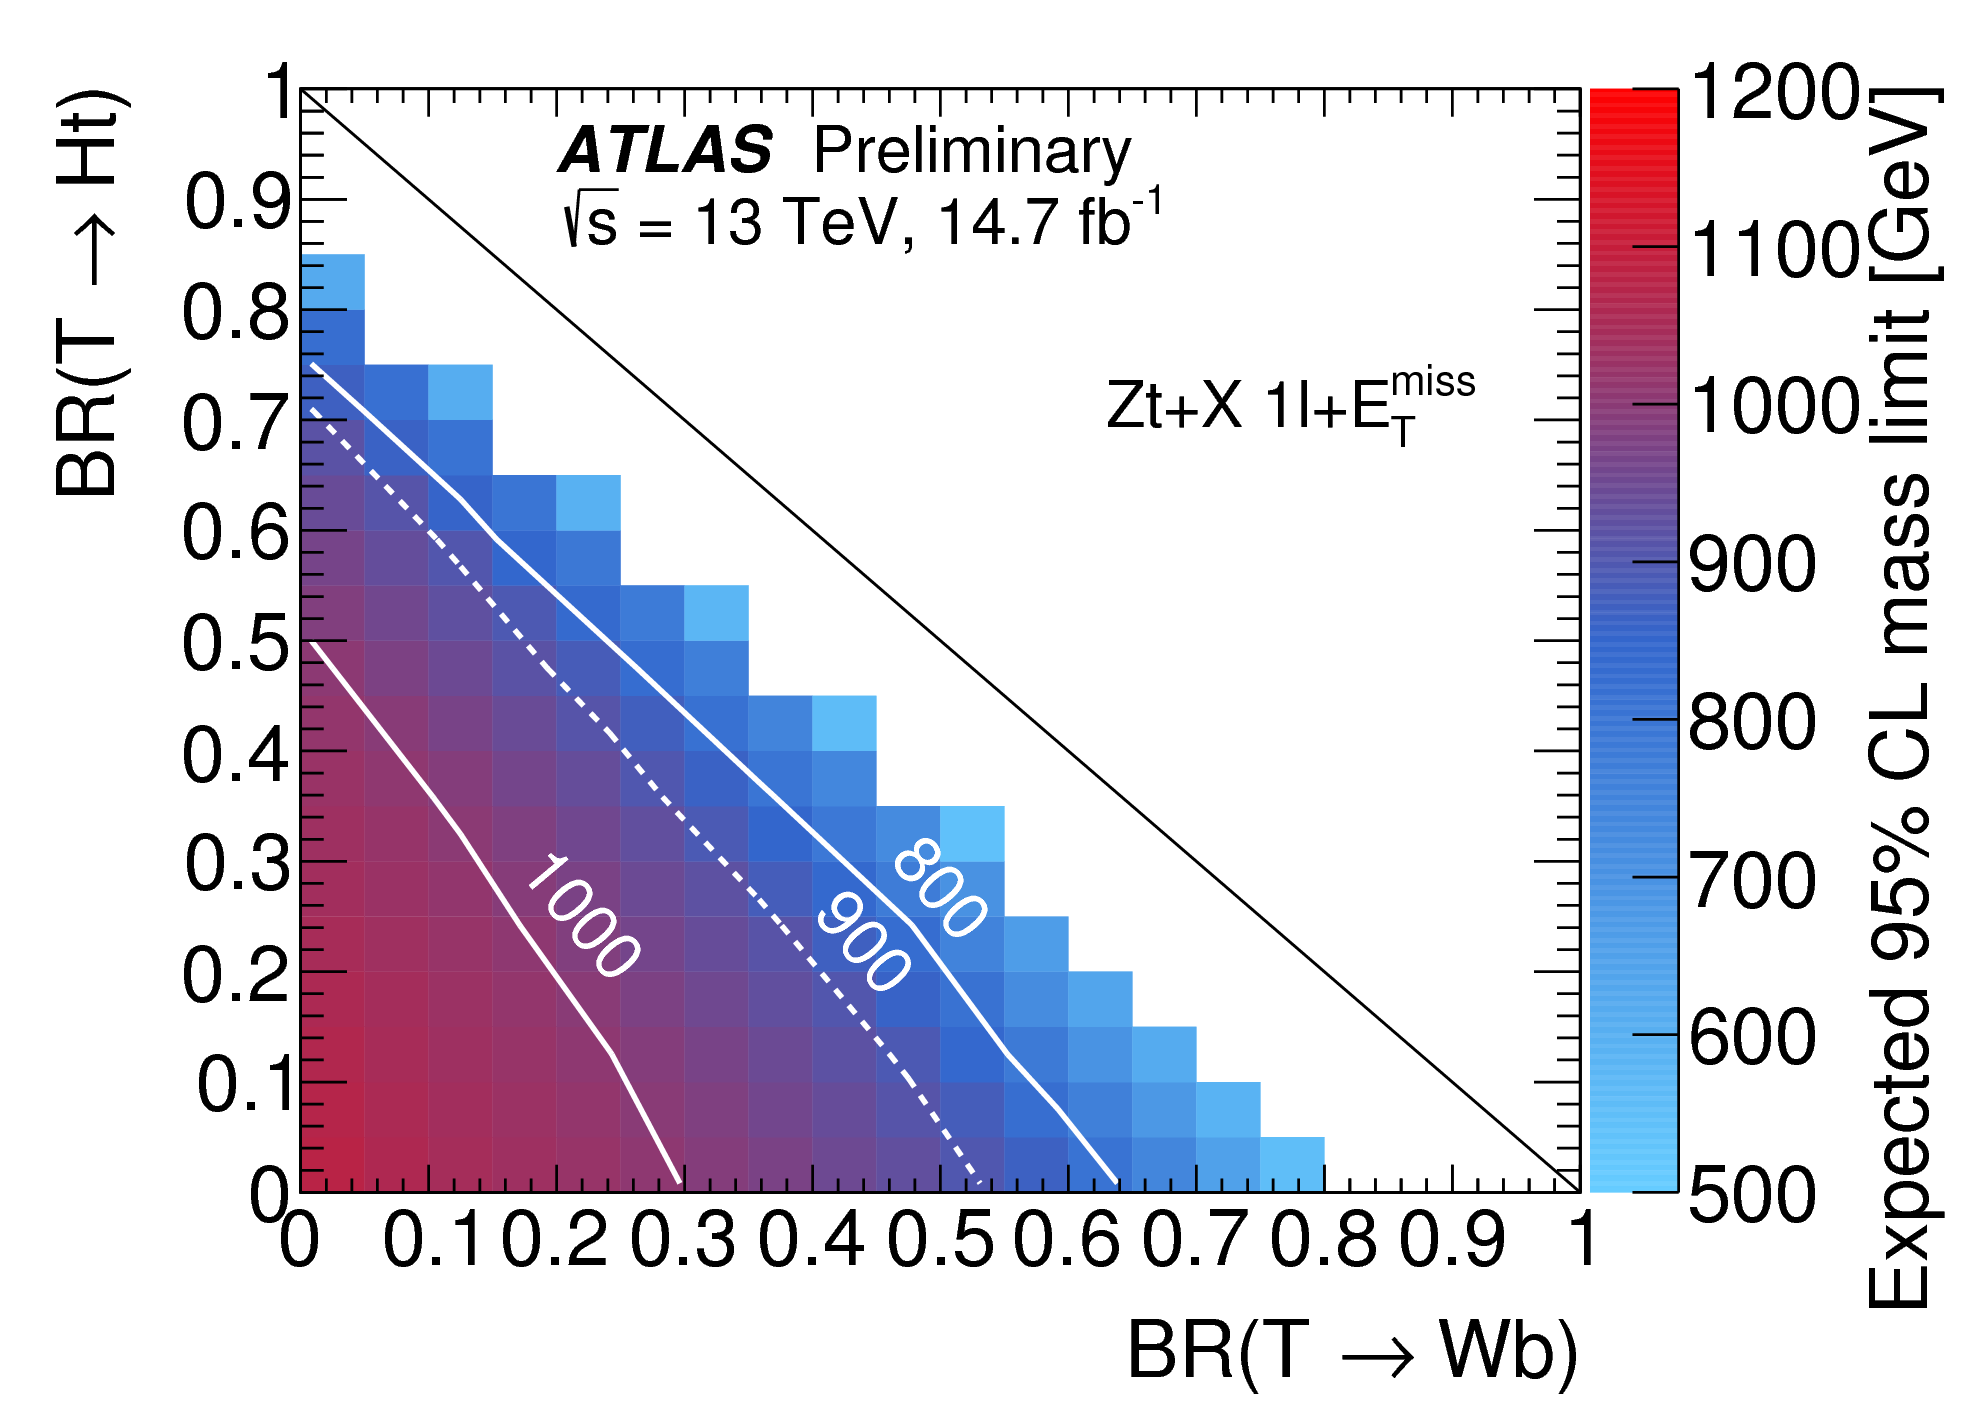
\includegraphics[width=0.9\textwidth]{figures/VLQ/Zta.png}
  \caption{}
  \label{}
\end{subfigure}
\captionsetup{width=0.85\textwidth} \caption{\small (a) Observed and (b) expected limit (95\% CL) on the mass of the $T$ quark in the plane 
of ${\rm BR}(T \to Ht)$ versus ${\rm BR}(T \to Wb)$ for the $Zt+X$ search. 
Contour lines are provided to guide the eye.}
\label{sec:vlq:fig:Zt}
\end{figure}


\begin{figure}[h!]
\begin{subfigure}{0.5\textwidth}
  \centering
  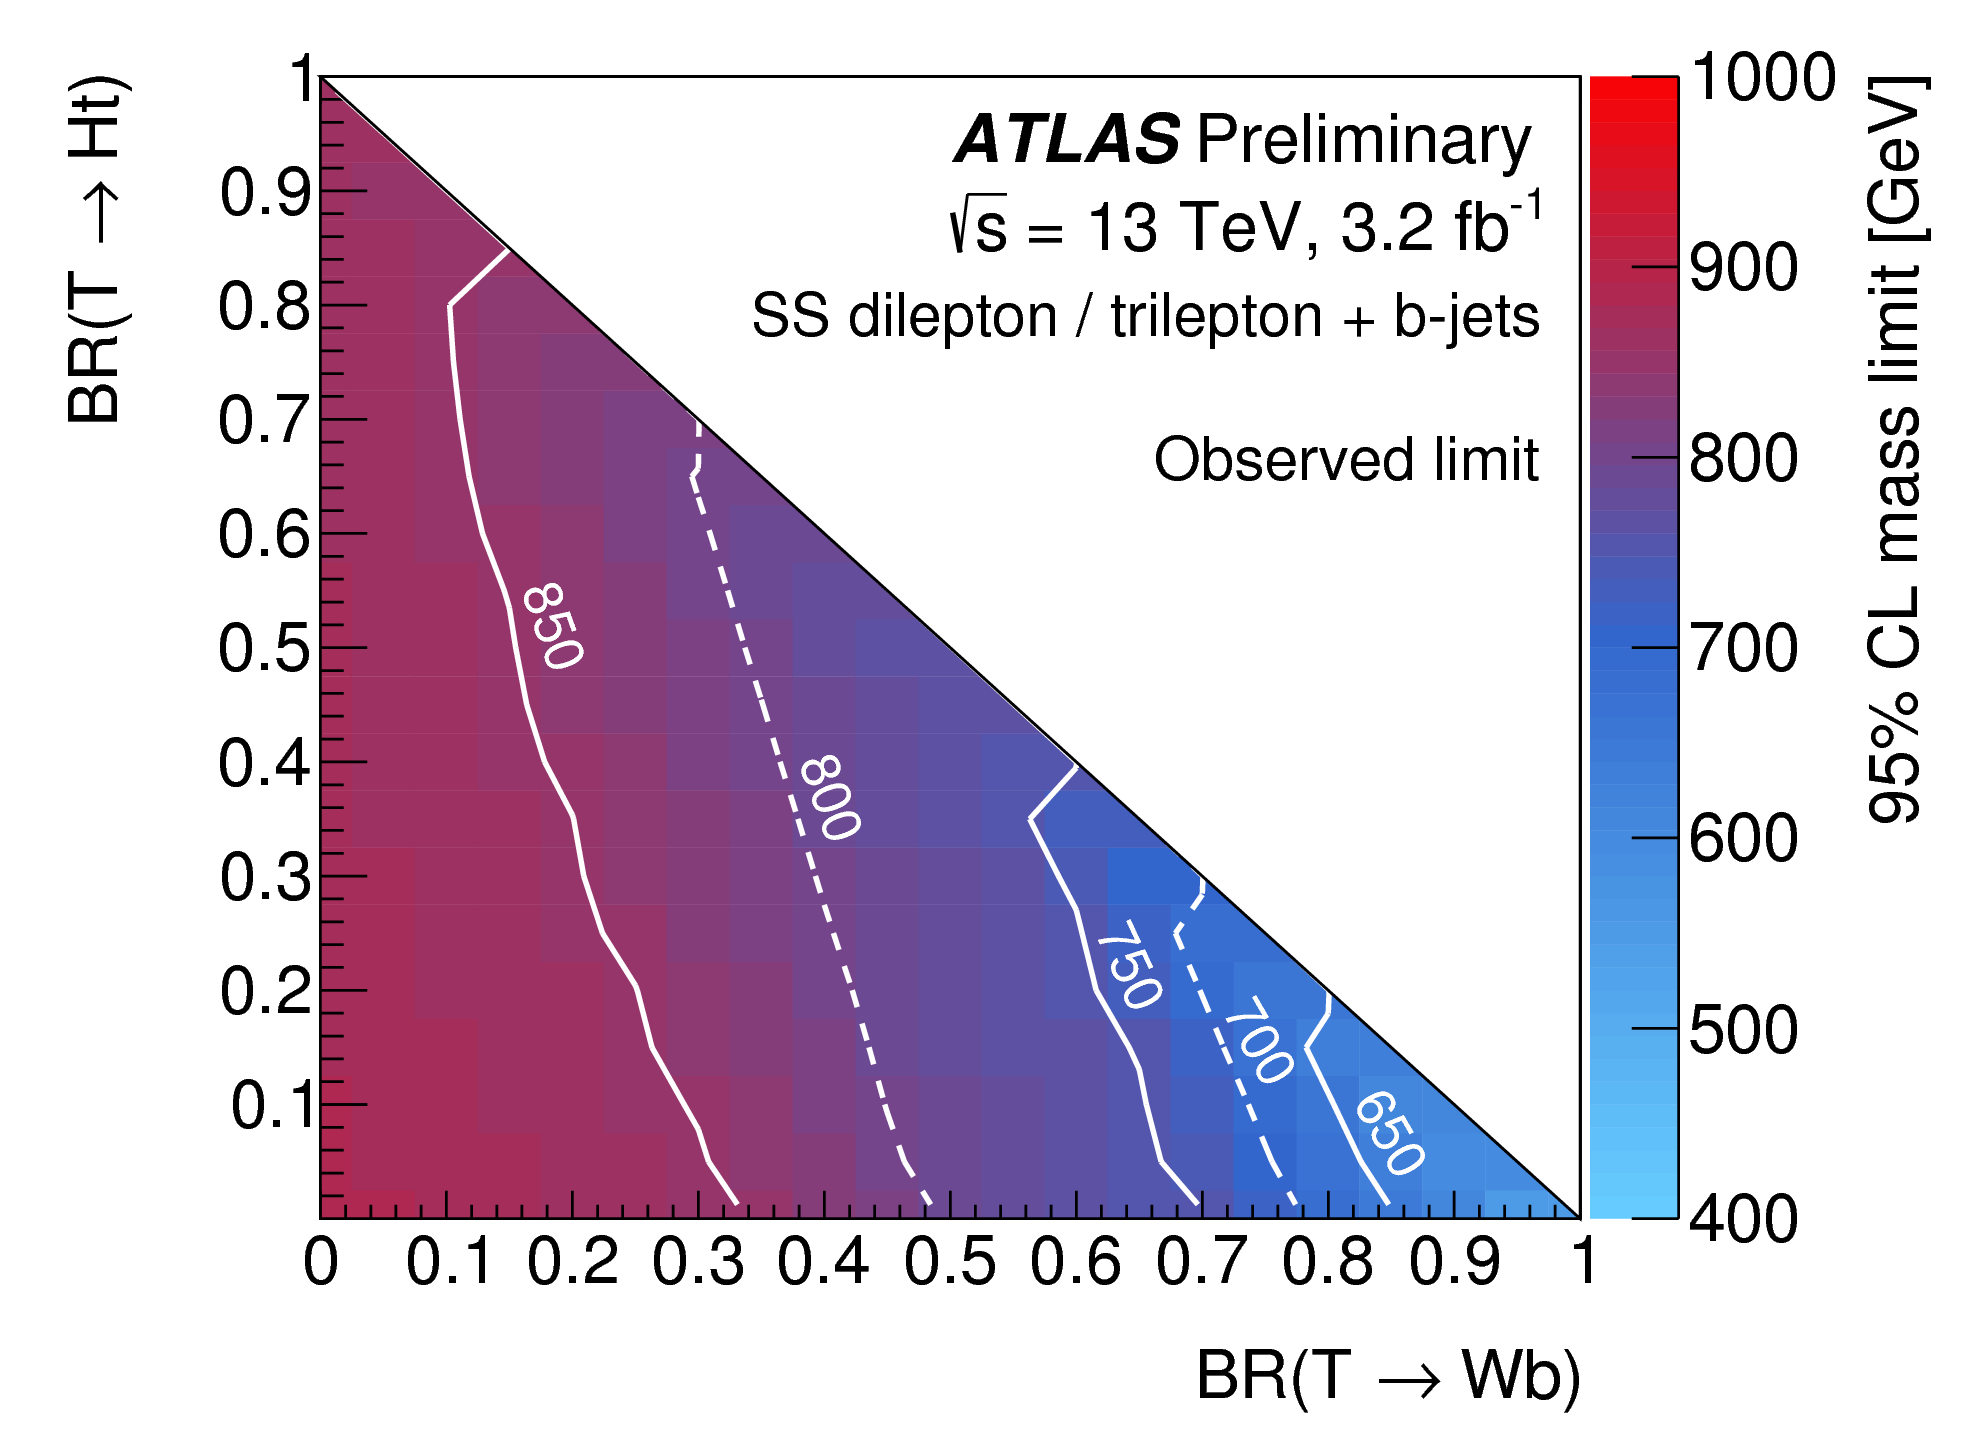
\includegraphics[width=0.9\textwidth]{figures/VLQ/ssb.png}
  \caption{}
  \label{}
\end{subfigure}
\begin{subfigure}{0.5\textwidth}
  \centering
  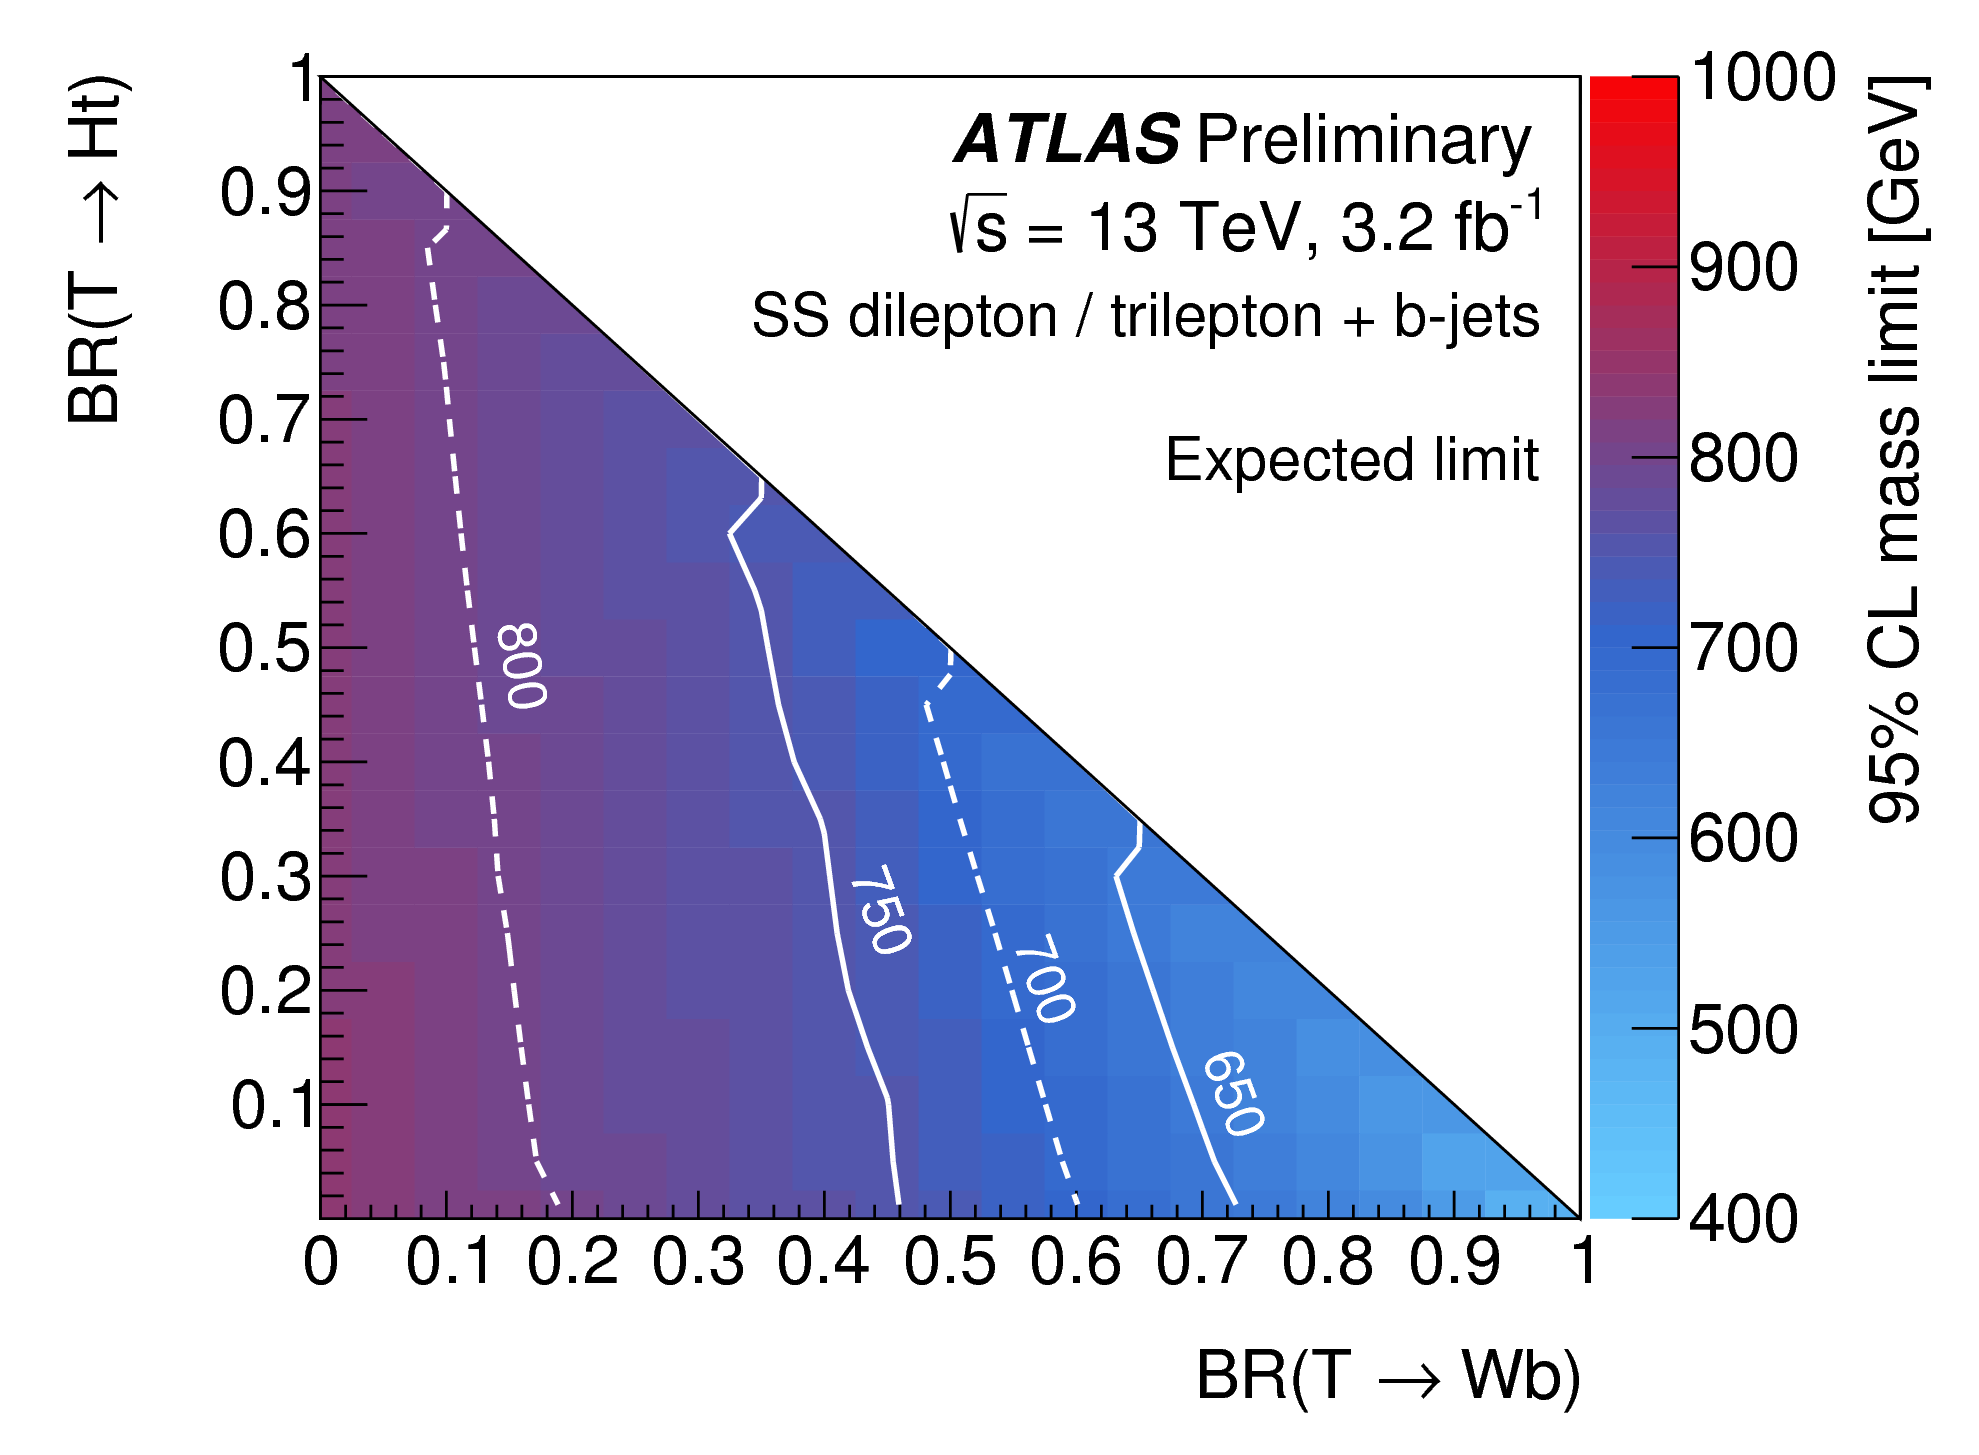
\includegraphics[width=0.9\textwidth]{figures/VLQ/ssa.png}
  \caption{}
  \label{}
\end{subfigure}
\captionsetup{width=0.85\textwidth} \caption{\small (a) Observed and (b) expected limit (95\% CL) on the mass of the $T$ quark in the plane 
of ${\rm BR}(T \to Ht)$ versus ${\rm BR}(T \to Wb)$ for the same-charge dileptons/trileptons search. 
Contour lines are provided to guide the eye.}
\label{sec:vlq:fig:SS}
\end{figure}
